\documentclass{article}
\usepackage[a4paper,left=25mm,right=25mm,top=20mm,bottom=15mm]{geometry}
\usepackage[ngerman]{babel}   %   %Sprachunterstützung
\usepackage[utf8]{inputenc}   %Eingabecodierung
% \usepackage[T1]{fontenc}         %T1-Codierung Zeichensatz
\usepackage{amsmath}
\usepackage{amssymb}
\usepackage{amsfonts}

\usepackage{textcomp}
\usepackage{fancyhdr}
\usepackage{siunitx}
\usepackage{graphicx} 
\usepackage{minted}


\usepackage{caption}
\newenvironment{code}{\captionsetup{type=listing}}{}
\usepackage[bookmarksopen=true]{hyperref}
\usepackage{float}
\usepackage{listings} % Für den Code
\usepackage{changepage} % Für geingerückte Blöcke mit adjustwidth

\usepackage[backend=bibtex,style=ieee]{biblatex}
\addbibresource{literatur.bib}

\usepackage{enumitem}
\usepackage{wasysym}
\usepackage{multicol} 
\usepackage{lmodern}
\usepackage{xcolor}
\usepackage{helvet}
\usepackage{tabularx}
\usepackage{eurosym}
\usepackage[htt]{hyphenat}
\usepackage{circuitikz}
\usepackage{tikz}
\usepackage{longtable}
\usepackage{mdframed} % für Text Boxen


\usepackage{pdfpages} % Required for including external PDF pages
\usepackage{pdflscape} % Required for landscape environment

\usetikzlibrary{arrows,automata}
\usepackage{tikz-timing}
\usetikztiminglibrary[rising arrows]{clockarrows}
\usepackage{array,cellspace}
\usepackage{wrapfig}


\newcommand{\boldinline}[1]{\textbf{\mintinline{sh}|#1|}}

\newcolumntype{L}[1]{>{\raggedright\arraybackslash}p{#1}} % linksbündig mit Breitenangabe
\newcolumntype{C}[1]{>{\centering\arraybackslash}p{#1}} % zentriert mit Breitenangabe
\newcolumntype{R}[1]{>{\raggedleft\arraybackslash}p{#1}} % rechtsbündig mit Breitenangabe
\newcolumntype{Y}{>{\centering\arraybackslash}X}
\newcolumntype{B}{>{\raggedright\arraybackslash}X}
\parskip=6pt
\setlength{\parindent}{0pt} 

\renewcommand{\arraystretch}{2.0}
\pagestyle{fancy}
\lfoot[\thepage]{SS 2024}
\rfoot[SS 2024]{\thepage}
\cfoot[]{ESP}

\rhead[]{\leftmark}
\lhead[\leftmark]{}

% \renewcommand{\familydefault}{\sfdefault}

% Set global options for minted
\setminted{
	breaklines,
	breakanywhere=false,
	linenos,
	xleftmargin=20pt
}

% evtl mintline line breaks ausmachen, aber nur wenn möglich vorher den line break zu machen 
%\setmintedinline{
%	breaklines=false,
%	breakanywhere=false
%}

\begin{document}
\begin{titlepage}
\thispagestyle{empty} % Keine Seitenzahl
\centering
    % \includegraphics[width=0.15\textwidth]{pic/thlogo/logo_TH-Koeln_CMYK_22pt.pdf}\par\vspace{1cm}

	{\Large I M A \par}
	{\huge\bfseries Intelligent Magic Audio\par}
	{Jonas Lux, Szymon Banasiak, Leon Braungardt\par}
	\vspace{2cm}
	{\Large\itshape Ein Projekt aus dem Modul ESP an der TH Köln im \par}
	{\Large\itshape Sommersemester 2024 \par}
	
	\vspace{4.5cm}
	\begin{figure}[h!]
		\centering
		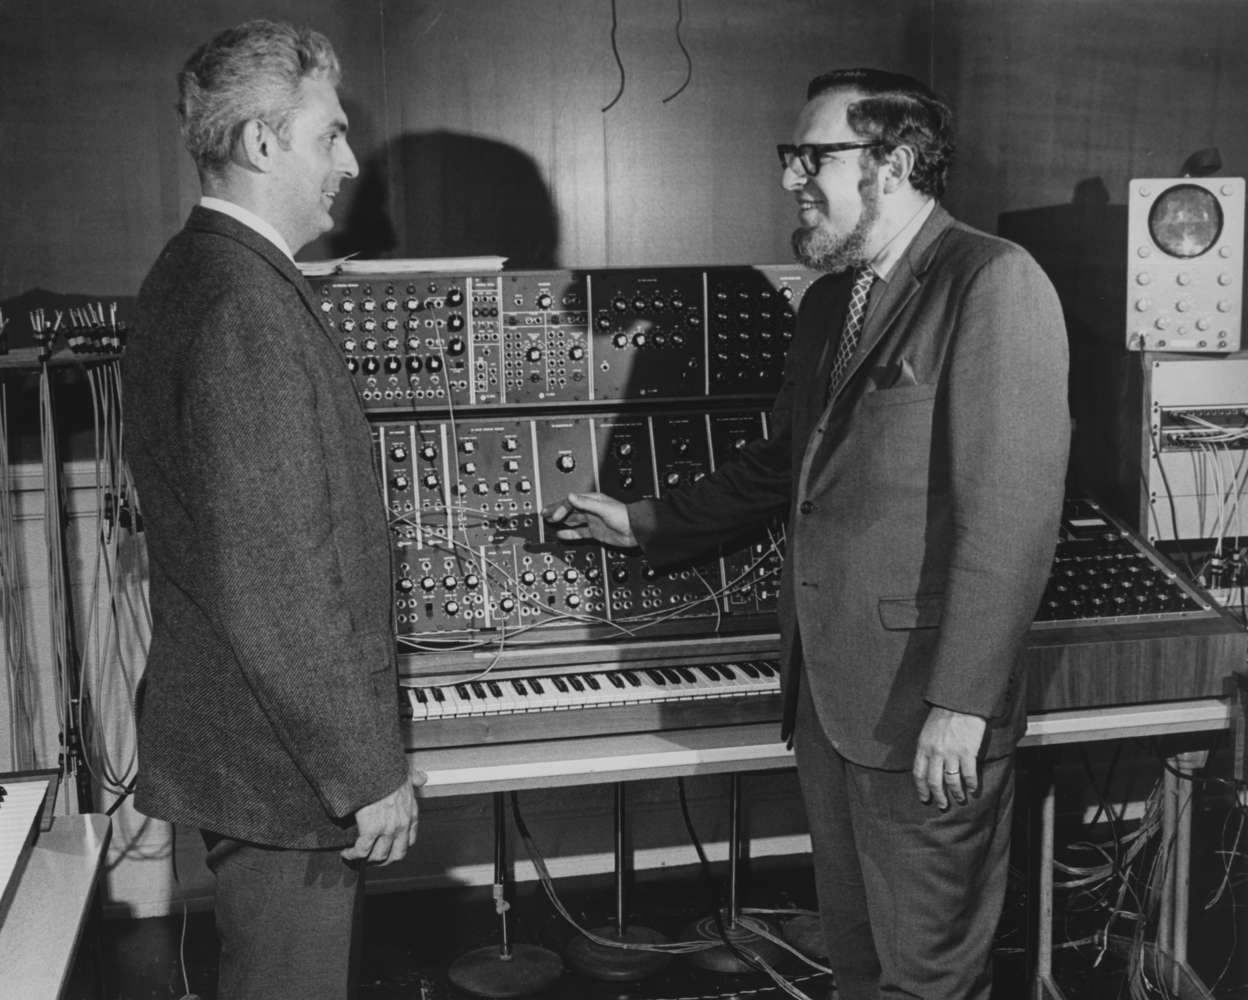
\includegraphics[width=0.45\textwidth]{images/titelbild-xD.jpg}
		\label{fig:img-input-data-graph}
	\end{figure}
	\vfill
	
	
	
  
\end{titlepage}

\addtocontents{toc}{\protect\thispagestyle{empty}}
\tableofcontents
\thispagestyle{empty}
\newpage
\listoffigures
\thispagestyle{empty} % Keine Seitenzahl
\newpage
\pagestyle{fancy}
\setcounter{page}{1} % Beginne Seitenzahl bei 1
%%%%%%%%%%%%%%%%%%%%%%%%%%%%%%%
\newpage
\section{Einleitung}

Bei dem Projekt ``Intelligent Magic Audio`` (IMA) handelt es sich um ein Projekt aus dem Modul ``Embedded Systems Praktikum`` (ESP) im Sommersemester 2024 an der TH Köln.

Ziel des Projekts ist die Entwicklung eines Audiosamplers im Eurorack-Standard, der auf einem STM32 Mikrocontroller basiert. Die Besonderheit des Samplers darin, dass auf eine SD-Karte geladenene Audiosamples über ein lokal laufendes Neuronales Netz (Edge AI) in fünf Klassen klassifiziert werden. Mit Hilfe von fünf Fadern und einer Suchfunktion kann der Nutzer sich passende Samples aus seiner Audiobibliothek vorschlagen lassen. 

Das Projektthema wurde dem betreuenden Professor aus Eigeninitiative vorgeschlagen, da es zentrale Aspekte der eingebetteten Systeme wie die Signal- bzw. Audioverarbeitung und den Umgang mit Peripheriegeräten vereint. Dies ermöglicht den Teammitgliedern, ihre Kenntnisse aus dem Modul ``Embedded Systems`` (ES) zu nutzen, um ein eigens entworfenes Produkt zu entwickeln und gleichzeitig ihre Fähigkeiten in ihren persönlichen Interessensgebieten zu vertiefen. Die Integration der Edge AI-Komponente bietet zudem die Möglichkeit, Erfahrungen im Betrieb neuronaler Netze auf Mikrocontrollern zu sammeln.


\newpage
\section{Detaillierte Projektbeschreibung}

	\subsection{Modulare Eurorack Synthesizer}
	
	In der modernen elektronischen Musikproduktion erfreut sich die Modularität von Synthesizern wieder großer Beliebtheit. 
	Die Methoden, verschiedene Module von unterschiedlichen Herstellern miteinander zu kombinieren, erleben ein Revival. \cite{ferguson2015interview}
	Wo einst die Reise der elektronischen Musik begann, werden diese Ansätze erneut aufgegriffen.
	
	In den 1950er Jahren erzeugten die Pioniere der elektronischen Musik mit Labor- und Testequipment neue Klänge. 
	Signalgeneratoren, Filter und anderes technisches Gerät aus den Ingenieurlabors wurden funktional zu Musikinstrumenten umgewandelt – die elektronische Musik war geboren. \cite{holmes2002electronic}
	
	In den 1990er Jahren, durch die bessere Zugänglichkeit und günstigeren Kosten von Chips und Halbleitern, fand dieses Mindset den Weg zu den Consumer-Musikproduzenten - Dieter Doepfer entwickelte den Eurorack-Standard für modulare Synthesizer. \cite{eurorack-standard}
	
	Die Module sind in 3U-Höhe (etwa 133,4 mm) und variabler Breite in HP (horizontal pitch) erhältlich, wobei 1 HP etwa 5,08 mm entspricht. Diese Maße basieren auf dem 19"-Rack-Standard, der in Computertechnik und Audio Equipment weit verbreitet ist. Die Module werden in Racks oder Cases montiert, die mit Schienen ausgestattet sind, um eine flexible und modulare Konfiguration zu ermöglichen. \cite{iec60297-3-108:2014}
	
	
	\begin{figure}[h!]
		\centering
		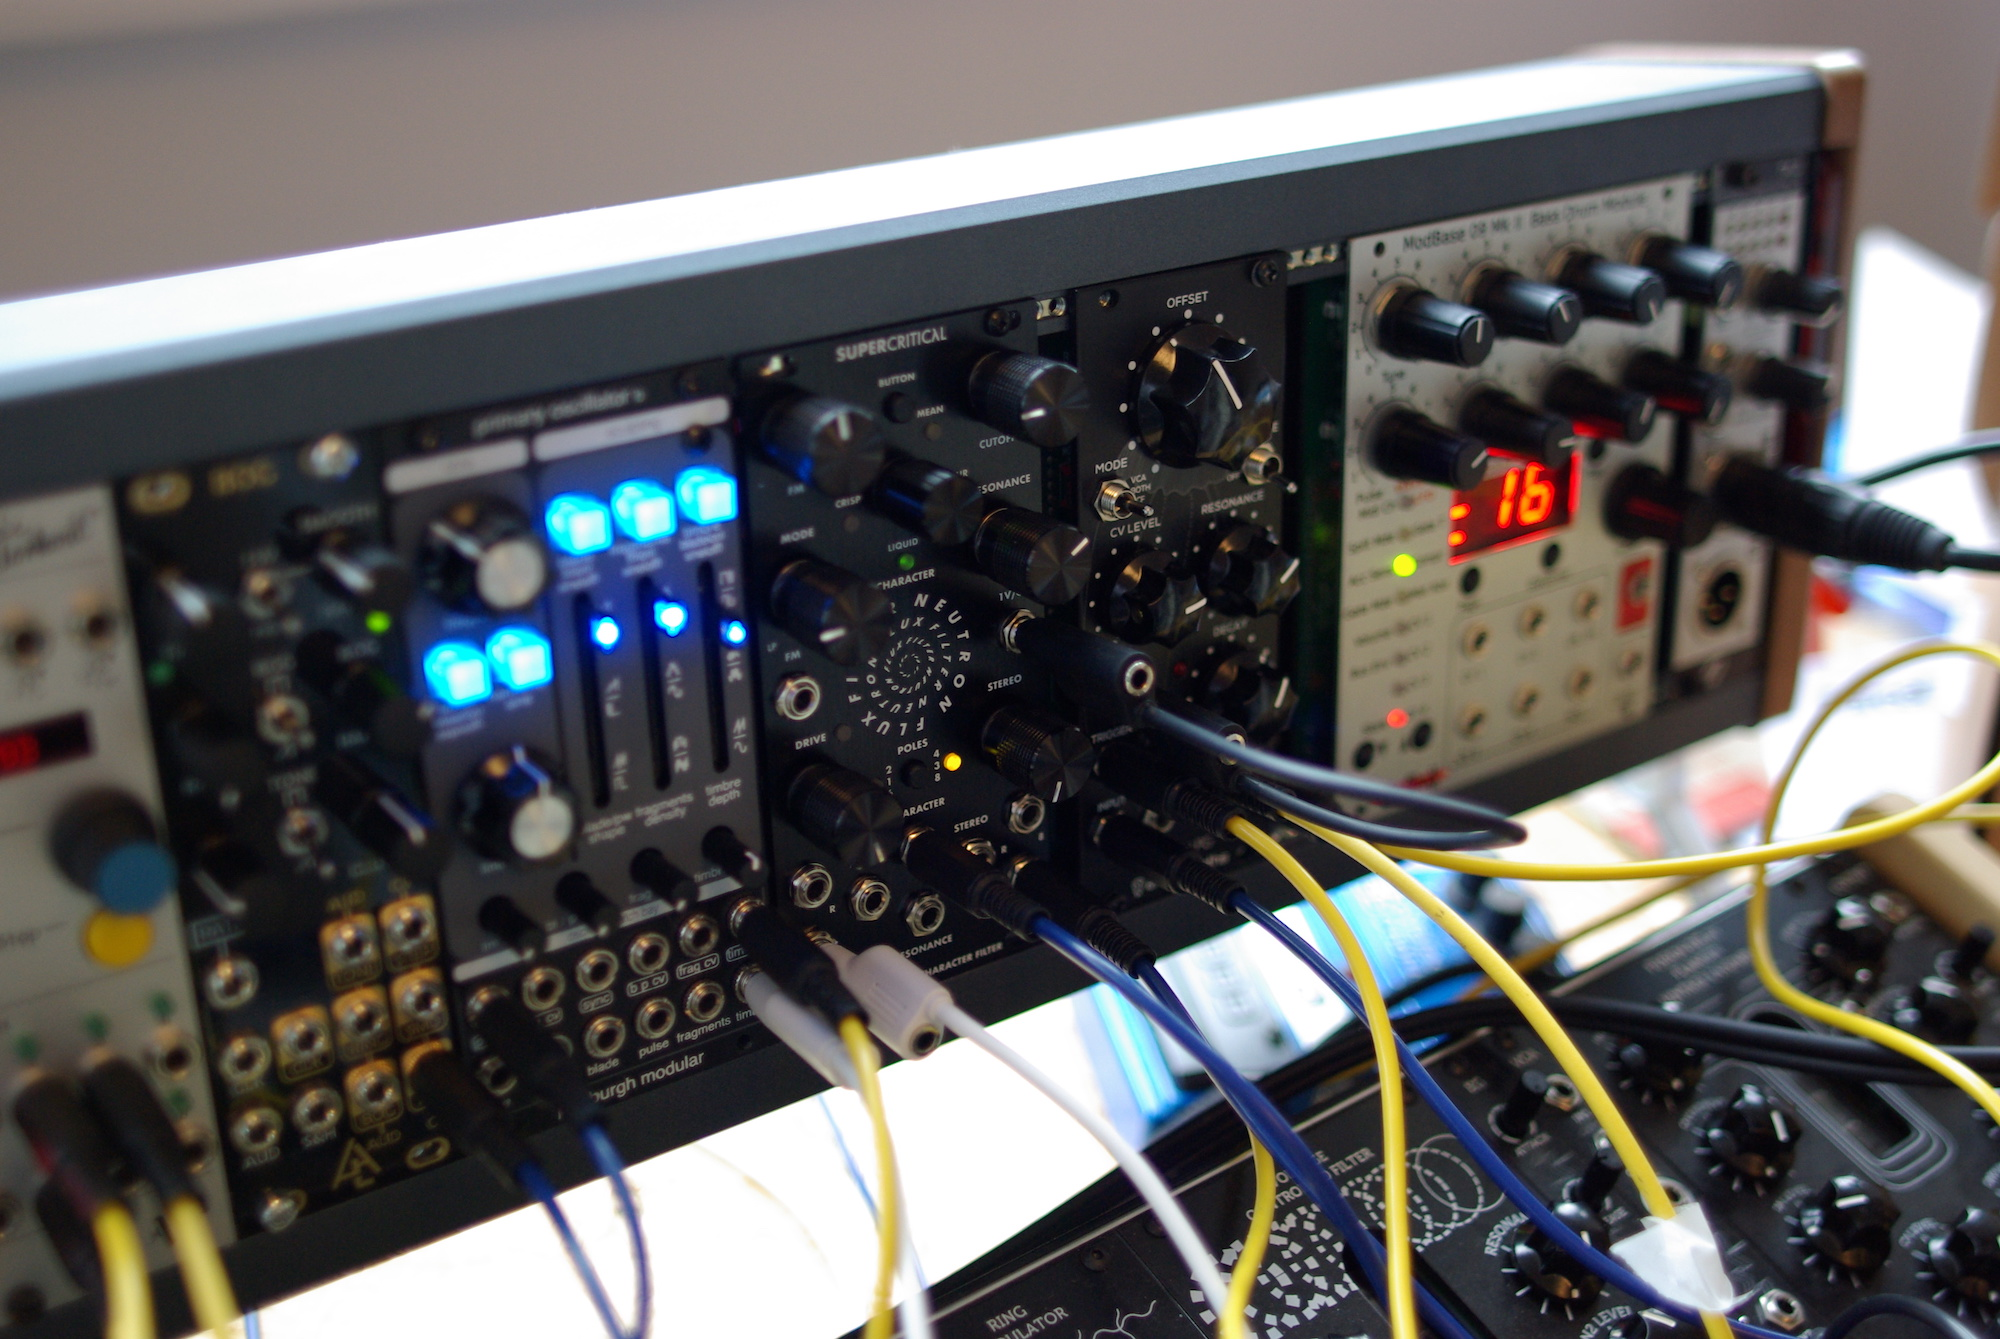
\includegraphics[width=0.5\textwidth]{images/02_detaillierte-projektbeschr/eurorack-patched}
		\caption{Gepatchtes Eurorack 3U Rack (einreihig)}
		\label{fig:eurorack-patched}
	\end{figure}
	
	Elektrisch werden Eurorack-Module über eine gemeinsame Stromversorgung betrieben, die typischerweise +12V, -12V und manchmal +5V bereitstellt. Module werden über 10-polige oder 16-polige Flachbandkabel an eine Stromverteilungsplatine (Bus Board) angeschlossen. Die wichtigsten elektrischen Verbindungen umfassen +12V, -12V und GND, wobei der 16-polige Anschluss zusätzlich +5V und weitere Signale unterstützen kann. \cite{eurorack-standard}
	
	Für die Signalübertragung nutzen Eurorack-Module 3,5 mm Monoklinkenstecker, um die Module miteinander zu ``verpatchen``. Über diese Kabel werden Audiosignale (typischerweise ±5V), Steuersignale (CV) und Triggersignale (0V bis +5V) zwischen den Modulen übertragen.
	
	Audiosignale, Steuersignale und Triggersignale werden also mit denselben Buchsen und Kabeln verbunden.
	Dies eröffnet enorme Möglichkeiten, die Klangpalette zu erweitern. So können beispielsweise Audiosignale zur Steuerung der Parameter eines Moduls verwendet werden, was kreative und innovative Patches ermöglicht.
	
	Mit der Eurorack Revolution haben sich modulare Synthesizer auch technisch weiterentwickelt. 
	Es wird vermehrt auf digitale Module gesetzt. 
	Die Zeit der Analog-Puristen ist vorbei; alle Möglichkeiten der digitalen Signalverarbeitung werden genutzt, um innovative Module zu entwerfen, die neue Methoden und Ideen in das eigene Rack bringen.
	
	Eine Unterkategorie der digitalen Module bilden die Audiosampler. Diese Module nehmen digitale Aufnahmen (Samples) von Klängen oder Musikstücken auf, speichern und spielen sie ab. Die Samples können durch verschiedene Trigger aktiviert und in unterschiedlichen Tonhöhen und Geschwindigkeiten abgespielt werden. 
	Audiosampler ermöglichen es Musikern, realistische Klänge von Instrumenten, Stimmen oder Umweltgeräuschen in ihre Musik zu integrieren und kreativ zu manipulieren.
	
	
	
	\newpage
	\subsection{Das Konzept}
	
	Es gibt durchaus Audiosampler mit ergonomischer Steuerung, großen hochauflösenden Displays und zahlreichen Knöpfen, um diese komplexen Audiomaschinen angenehm zu steuern. 
	Beispiele hierfür sind die legendäre MPC von AKAI oder der Octatrack von Elektron. 
	
	Die Hardware dieser Geräte sind jedoch aufgrund ihrer Bedienelemente und der damit einhergehenden Ergonomie so groß, dass sie unmöglich in ein Eurorack unterzubringen sind.
	
	\begin{wrapfigure}{r}{0.4\textwidth} % Increase the width of the figure environment
		\vspace{-20pt + 0.02\textwidth}
		\hspace{0.02\textwidth} % Add horizontal space
		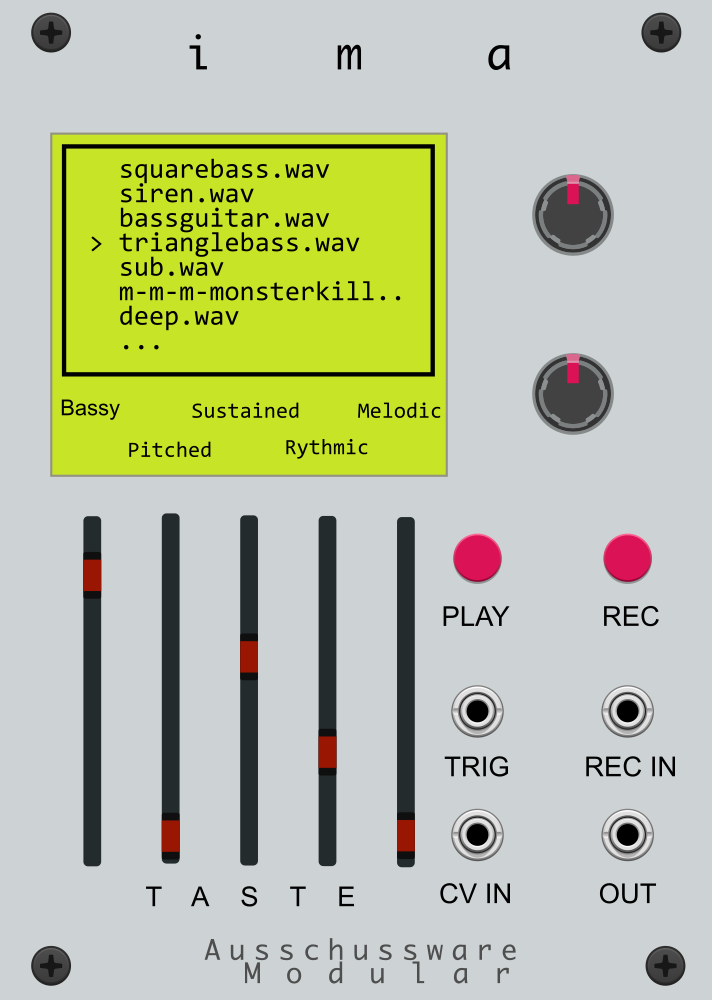
\includegraphics[width=0.38\textwidth]{images/02_detaillierte-projektbeschr/ima_mockup.png} % Keep the image size the same
		\caption{Panel Design Mockup }
		\label{fig:panel_mockup}
		\vspace{-20pt}
	\end{wrapfigure}

	Daher sind Samplermodule im Eurorack-Standard häufig mit wenigen Features ausgestattet oder haben aufgrund der minimalen Bedienelemente eine komplizierte, verschachtelte Bedienung mit vielen Untermenüs und Ebenen. 
	
	``\textbf{I M A}`` (Intelligent Magic Audio) macht es Musikern und Sounddesignern hier deutlich einfacher! Der Schlüsselpunkt ist das gezielte Finden von Samples aus dem vorhandenen persistenten Speicher. Nur Samples des gewünschten Typs zu filtern, setzt normalerweise ein hohes Maß an manueller Sortierung und penibler Ordnerstrukturierung voraus.
	
	Durch den neuronalgesteuerten Suchfilter von I M A kann eine Vorauswahl anhand musikalischer Parameter getroffen werden, ohne den kreativen Fluss des Künstlers zu unterbrechen.
	
	Das Neuronale Netz klassifiziert jedes neu hinzugefügte Audiosample nach 5 Klassen, welche speziell musikalischen Parametern entsprechen. Das ermöglicht einen, für den Musiker, organischen Suchvorgang.
	Die Klassifizierung wird nach der Aufnahme durch den \textbf{REC IN}, oder durch das manuelle Kopieren auf die SD Karte angestoßen, also immer wenn eine neue Audiodatei in den persistenten Speicher des Samplers hinzukommt.
	
	
	Wie in \textbf{\autoref{fig:panel_mockup}} ersichtlich, gibt es 5 Schieberegler (von nun an Fader genannt), sowie 2 Encoder.
	Der Suchfilter lässt sich über die 5 \textbf{``TASTE``} Fader einstellen. 
	Jeder Fader entspricht einer Klasse der Klassifizierung des Neuronalen Netzes.
	Je nach eingestelltem Suchfilter, werden Samples zum Abspielen vorgeschlagen, die den Suchfiltereinstellungen entsprechen.
	
	Ist man beispielsweise auf der Such nach einem bassigen und flächigen Sample, stellt man die Fader entsprechend seiner Wünsche ein (viel \textit{Bassy} und \textit{Sustained}). 
	Ein Filteralgorithmus zeigt nun den Suchfilter entsprechenden Samples auf dem Display an.
	Nun kann ein Sample mit dem Encoder ausgewählt werden, und per Druck auf den Encoder, oder per Impuls über den \textbf{TRIG IN} abgespielt werden. 
	
	
	
	
	
	

\newpage
\section{Projektanforderungen}

TODO: Nummerierung der LFs

Basierend auf dem zuvor entwickelten Produktkonzept wurden funktionale und nicht-funktionale Anforderungen abgeleitet. Sie bilden das Lastenheft des Projekts und werden in den folgenden zwei Abschnitten näher beschrieben.

\subsection{Funktionale Anforderungen}
Die funktionalen Anforderungen definieren die Funktionen, die dem Benutzer zur Verfügung gestellt werden sollen. Jede dieser Anforderungen wird mit dem Kürzel „LF“ für Lastenfall, gefolgt von einer fortlaufenden Nummer, gekennzeichnet.

\subsubsection{LF1: Steuerung des Cursors und Auswahl eines Samples}
	\hypertarget{LF01_Link}{}
\begin{longtable}[c]{|p{3cm}|p{13cm}|}
	\hline
	\textbf{Priorität} & Muss \\
	\hline
	\textbf{Akteur} & Benutzer \\
	\hline
	\textbf{Beschreibung} & 
	\begin{tabularx}{13cm}{X}
		\textbf{1. Cursor Bewegung:} \\
		\textbf{Aktion:} Der Benutzer dreht den Encoder. \\
		\textbf{Reaktion:} Der Cursor auf dem LCD-Display bewegt sich nach oben oder unten entsprechend den Stepperschritten des Encoders. \\
		\textbf{Details:} \\
		- Der Cursor bewegt sich um eine Position in der Liste pro Schritt des Encoders. \\
		- Der Cursor kann den Beginn oder das Ende der Liste erreichen, ohne die Liste über die Grenzen hinaus zu bewegen. Er spring von daher am Anfang oder Ende der Liste. \\
		\\
		\textbf{2. Sample Auswahl:} \\
		\textbf{Aktion:} Der Benutzer drückt den Switch des Encoders. \\
		\textbf{Reaktion:} Das aktuell ausgewählte Sample wird hervorgehoben und sein Name wird unter der Liste auf dem LCD-Display angezeigt. \\
		\textbf{Details:} \\
		- Der Name des ausgewählten Samples wird deutlich unter der Liste angezeigt. \\
		- Der Name sollte in einem Format angezeigt werden, das gut lesbar ist und keine Abkürzungen oder Unklarheiten aufweist. \\
	\end{tabularx} \\
	\hline
\end{longtable}

\newpage
\subsubsection{LF2: Verhalten der Fader und des Displays}
	\hypertarget{LF02_Link}{}
\begin{longtable}[c]{|p{3cm}|p{13cm}|}
	\hline
	\textbf{Priorität} & Muss \\
	\hline
	\textbf{Akteur} & Benutzer \\
	\hline
	\textbf{Beschreibung} & 
	\begin{tabularx}{13cm}{X}
		\textbf{1. Anzeige der Fader-Werte:} \\
		\textbf{Aktion:} Der Benutzer bewegt die Schiebepotentiometer. \\
		\textbf{Reaktion:} Die prozentuale Angabe der Spannung, in der sich der Potentiometer befindet, wird angezeigt. \\
		\textbf{Details:} \\
		- Die prozentualen Ausgaben spiegeln die Klassen wider, wie Rhythmic, Sustained, usw., sowie die Einstellung des Threasholds \\
		- Die Prozentsätze sollen klar und deutlich angezeigt werden, ohne Verzögerung. \\
		\\
		\textbf{2. Filtern der Samples:} \\
		\textbf{Aktion:} Der Benutzer bewegt die Schiebepotentiometer. \\
		\textbf{Reaktion:} In der Liste auf dem Display werden die Samples angezeigt dessen Audio Klassen nach der Klassiefiezierung, die den Prozentsatz der Potentiometereinstellung nicht mehr als einen bestimmten Schwellenwert überschreiten. \\
		\textbf{Details:} \\
		- Die Anzeige der Samples soll dynamisch aktualisiert werden, basierend auf den aktuellen Fader-Werten. \\
		- Der Schwellenwert kann angepasst werden, um eine präzise Filterung der Samples zu ermöglichen. \\
	\end{tabularx} \\
	\hline
\end{longtable}
\subsubsection{LF03: Klassifizierung von Audiodateien des Benutzers durch ein neuronales Netz}
\label{lf-nn-01}

\begin{table}[h!]
	\begin{tabularx}{\textwidth}{|l|X|}
		\hline
		\textbf{Priorität} & Muss \\ \hline
		\textbf{Akteur} & Benutzer \\ \hline
		\textbf{Beschreibung} & Ein neuronales Netz soll beim Einschalten des Samplers die unklassifizierten Audiosamples in für die Musikproduktion relevante Kategorien klassifizieren, wie beispielsweise Genre, Instrumententyp oder Klangfarbe.
		
		Dieser Lastenfall enthält drei Arbeitspakete:
		\begin{enumerate}
    		\item \textbf{/LF03/AP01 Auswahl geeigneter Merkmalsklassen für Audiosamples}: Diese Kategorien sollten zum einen sinnvoll bei der Musikproduktion sein, zum anderen auch mit der genutzten Hardware klassifizierbar und damit realistisch sein.
    		\item \textbf{/LF03/AP02 Entwicklung und Training des neuronalen Netzes}: Das neuronale Netz muss in der Lage sein, annährend zutreffende Klassifizierungsergebnisse auszugeben. Ziel ist ein Accuracy-Wert von über 50\%. Zum Vergleich läge der Accuracy-Wert bei \textit{$\frac{1}{5} = 20\%$}, wenn das neuronale Netz rein zufällige Ergebnisse ausgeben würde. Gleichzeitig ist dieses Ziel von 50\% realistisch erreichbar. Um dieses Ziel zu erreichen, muss das neuronale Netz ausreichend mit relevanten Daten trainiert werden. Weiterhin sollte die Confusion-Matrix eine klare Tendenz in der korrekten Klassifizierung der Kategorien aufzeigen. Darüber hinaus sollten auch manuell eingegebene Samples, wie beispielsweise ein Rock-Song, zuverlässig den entsprechenden Kategorien zugeordnet werden können. 
			\item \textbf{/LF03/AP03 Betrieb des neuronalen Netzes auf dem Nucleo-F7 Board}: Das neuronale Netz, einschließlich aller vor- und nachgelagerten Datenvorverarbeitungsschritte und der Generierung der Spektrogramme, muss auf einem Nucleo-F7 Board laufen können. 
		\end{enumerate}
		\\ \hline
	\end{tabularx}
\end{table}
\subsubsection{LF04: Aufnahme von Audioquelle über REC IN}
Das System muss eine Audioquelle, welche in der Eingangsbuchse eingesteckt ist aufnehmen können, und diese Aufnahme als korrekt kodierte PCM .wav Datei auf der SD-Karte abspeichern. Nach der Aufnahme muss eine Indexierung und Klassifizierung durch das Neuronale Netz geschehen (Wie in LFxxx beschrieben)


\newpage

\subsection{Nicht-Funktionale Anforderungen}
Die nicht-funktionalen Anforderungen spezifizieren Qualitätsmerkmale, die das System erfüllen muss, aber nicht direkt mit den spezifischen Funktionen verbunden sind. Diese Anforderungen werden mit dem Kürzel „LQ“, gefolgt von einer fortlaufenden Nummer, gekennzeichnet.


\subsubsection{Performance}

\begin{table}[h!]
	\begin{tabularx}{\textwidth}{|l|X|}
		\hline
		\textbf{/LQ1/} & \textbf{Latenz} \\ \hline
		\textbf{Kategorie} & Performance \\ \hline
		\textbf{Beschreibung} & Die Latenzzeit zwischen dem Triggern des Abspielmechanismus (Play-Button oder TRIG IN) und der Audiowiedergabe soll minimal sein (unter \SI{20}{\milli\second}), um die Funktionalität als Musikinstrument für die Live-Performance zu gewährleisten. \\ \hline
	\end{tabularx}
\end{table}

\begin{table}[h!]
	\begin{tabularx}{\textwidth}{|l|X|}
		\hline
		\textbf{/LQ2/} & \textbf{Performante Sampleklassifizierung} \\ \hline
		\textbf{Kategorie} & Performance \\ \hline
		\textbf{Beschreibung} & Das System muss in der Lage sein, Audio-Daten schnell zu Klassifizieren, damit der Nutzer nicht aus dem Kreativ-Fluss gezogen wird. \\ \hline
	\end{tabularx}
\end{table}

\begin{table}[h!]
	\begin{tabularx}{\textwidth}{|l|X|}
		\hline
		\textbf{/LQ3/} & \textbf{Datenübertragungsrate} \\ \hline
		\textbf{Kategorie} & Performance \\ \hline
		\textbf{Beschreibung} & Die Middleware muss hohe Datenübertragungsraten unterstützen, um eine kontinuierliche und verlustfreie Audioübertragung zu gewährleisten. \\ \hline
	\end{tabularx}
\end{table}

\subsubsection{Benutzerfreundlichkeit}

\begin{table}[h!]
	\begin{tabularx}{\textwidth}{|l|X|}
		\hline
		\textbf{/LQ4/} & \textbf{Intuitive Benutzeroberfläche} \\ \hline
		\textbf{Kategorie} & Benutzerfreundlichkeit \\ \hline
		\textbf{Beschreibung} & Die Benutzeroberfläche muss intuitiv und leicht bedienbar sein, damit Nutzer direkt damit arbeiten können, ohne eine Dokumentation lesen zu müssen. \\ \hline
	\end{tabularx}
\end{table}

\newpage
\subsubsection{Effizienz}

\begin{table}[h!]
	\begin{tabularx}{\textwidth}{|l|X|}
		\hline
		\textbf{/LQ5/} & \textbf{Optimierung der Audioverarbeitung} \\ \hline
		\textbf{Kategorie} & Effizienz \\ \hline
		\textbf{Beschreibung} & Algorithmen für die Audioverarbeitung und Klassifizierung sollten so optimiert sein, dass sie minimale Rechenressourcen benötigen, ohne die Genauigkeit zu beeinträchtigen. \\ \hline
	\end{tabularx}
\end{table}
\newpage
\section{Spezifikation}
Basierend auf dem entwickelten Konzept und den definierten Anforderungen wird die detaillierte Spezifikation des Systems ausgearbeitet. Diese umfasst die Architektur des gesamten Systems, welche die Aufteilung in einzelne Komponenten und deren Interaktion untereinander beschreibt. Ebenso wurden die Schnittstellen zwischen den Komponenten definiert. Weiterhin wird erläutert, wie das System mit seiner Umgebung interagiert. Die technische Spezifikation umfasst die verwendete Hardware sowie die eingesetzten Protokolle und Standards, die für Umsetzung der einzelnen Komponenten benötigt werden. 

Zur besseren Veranschaulichung des Gesamtsystems, Beziehungen zwischen den Komponenten und der Abläufe wurden, wo sinnvoll, Diagramme erstellt. Diese visualisieren bestimmte Zusammenhänge. Bei der Erstellung dieser Diagramme wurde das SA/RT-Entwurfskonzept als Orientierungshilfe genutzt. Aufgrund der des hohen Umfangs bzw. der Komplexität des Projekts wurden die strengen Vorgaben des SA/RT-Konzepts jedoch flexibel gehandhabt und nicht strikt befolgt.

\subsection{Architektur}
Die Architektur des Projekts bietet eine Gesamtdarstellung des Systems und zeigt, wie die verschiedenen Komponenten miteinander interagieren. Das System gliedert sich in drei Hauptbereiche: Audioverarbeitung, Benutzeroberfläche (User Interface) und das neuronale Netz.

\begin{itemize}
    \item Systemarchitektur: Gesamtdarstellung des Systems, wie Komponenten zusammenarbeiten
    \item Unterteilung in 3 Komponenten (Audio, User Interface, NN)
    \item Hier SA/RT Kontextdiagramm (evtl. ein Gesamt-Diagramm und pro Komponente ein weiteres)
    \item Hier SA/RT Modell für Zustandsautomat? und ggf. weitere Modelle
    \item Entwurfsmodell erläutern
    \item Alles auf einem NUCLEO F7 Board
    \item persistenter Datenspeicher der Audiodaten und deren Klassifizierungen in Struct auf SD-Karte
    
    \begin{figure}[H]
    	\centering
    	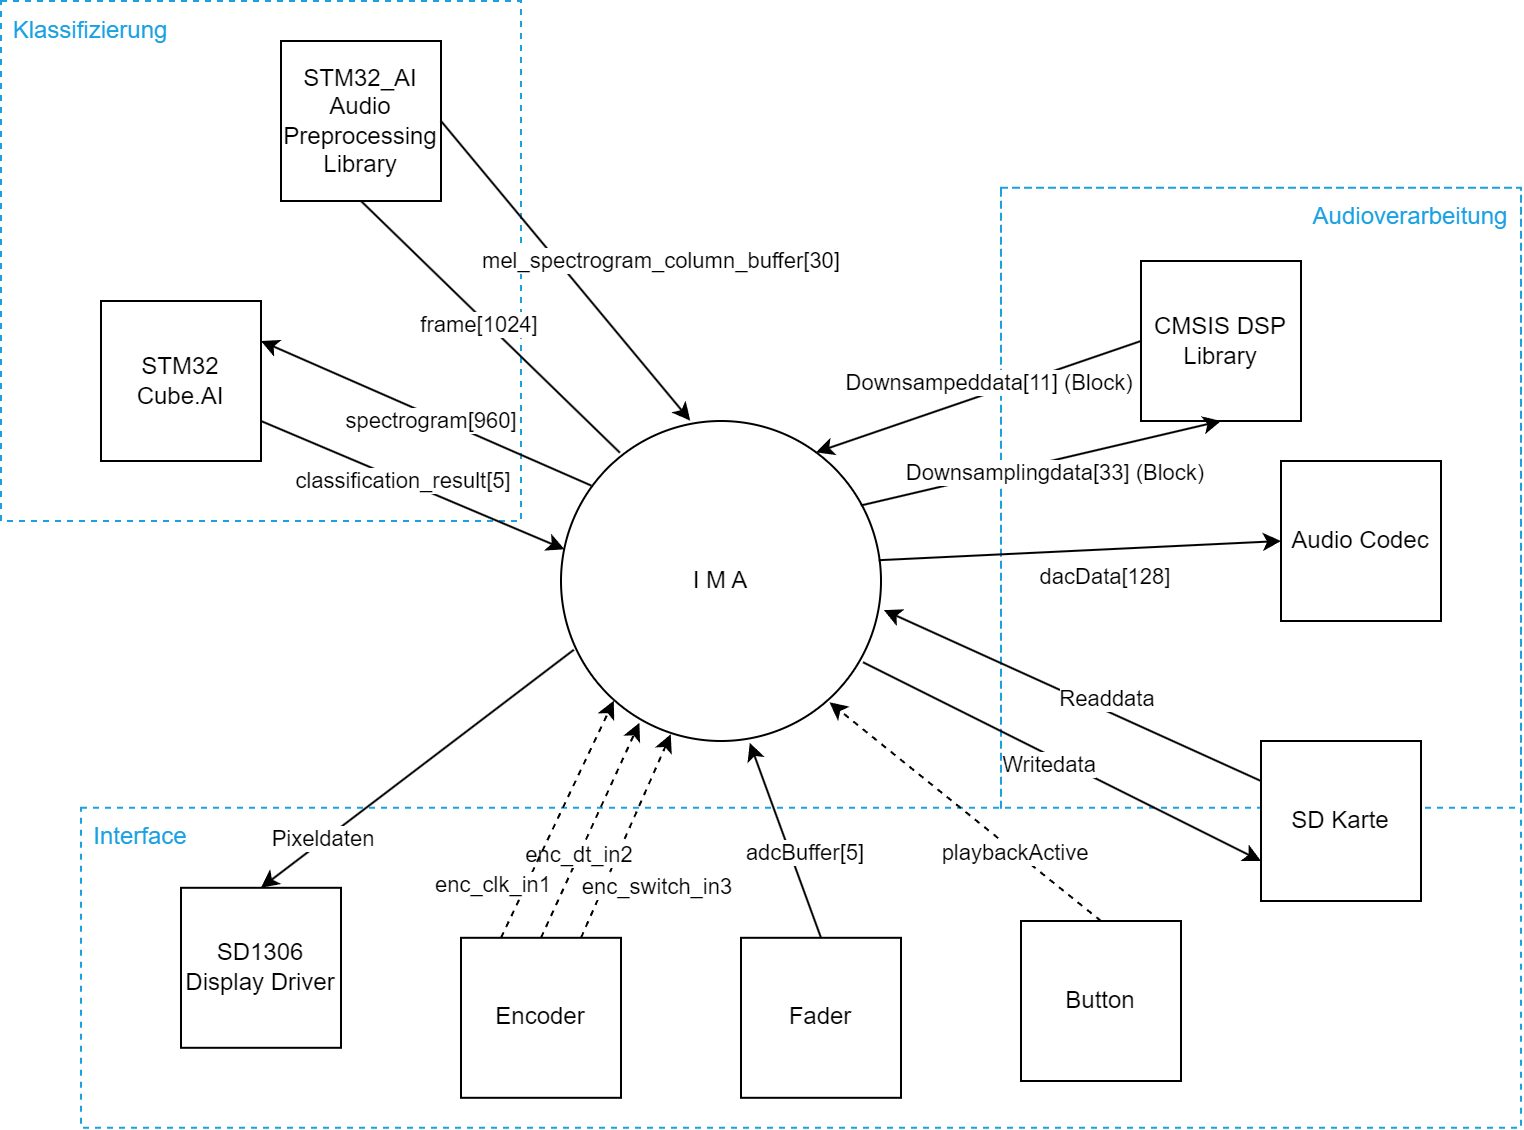
\includegraphics[width=0.8\textwidth]{images/04_spezifikation/kontextdiagramm_gesamt.drawio.png}
    	\caption{Kontextdiagramm des Gesamtsystems}
    	\label{fig:context_diagram_gesamt}
    \end{figure}
    
    %TODO: ausformulieren
    
    %TODO: Kontextdiagramme pro Untersystem
   
    
    \begin{figure}[H]
    	\centering
    	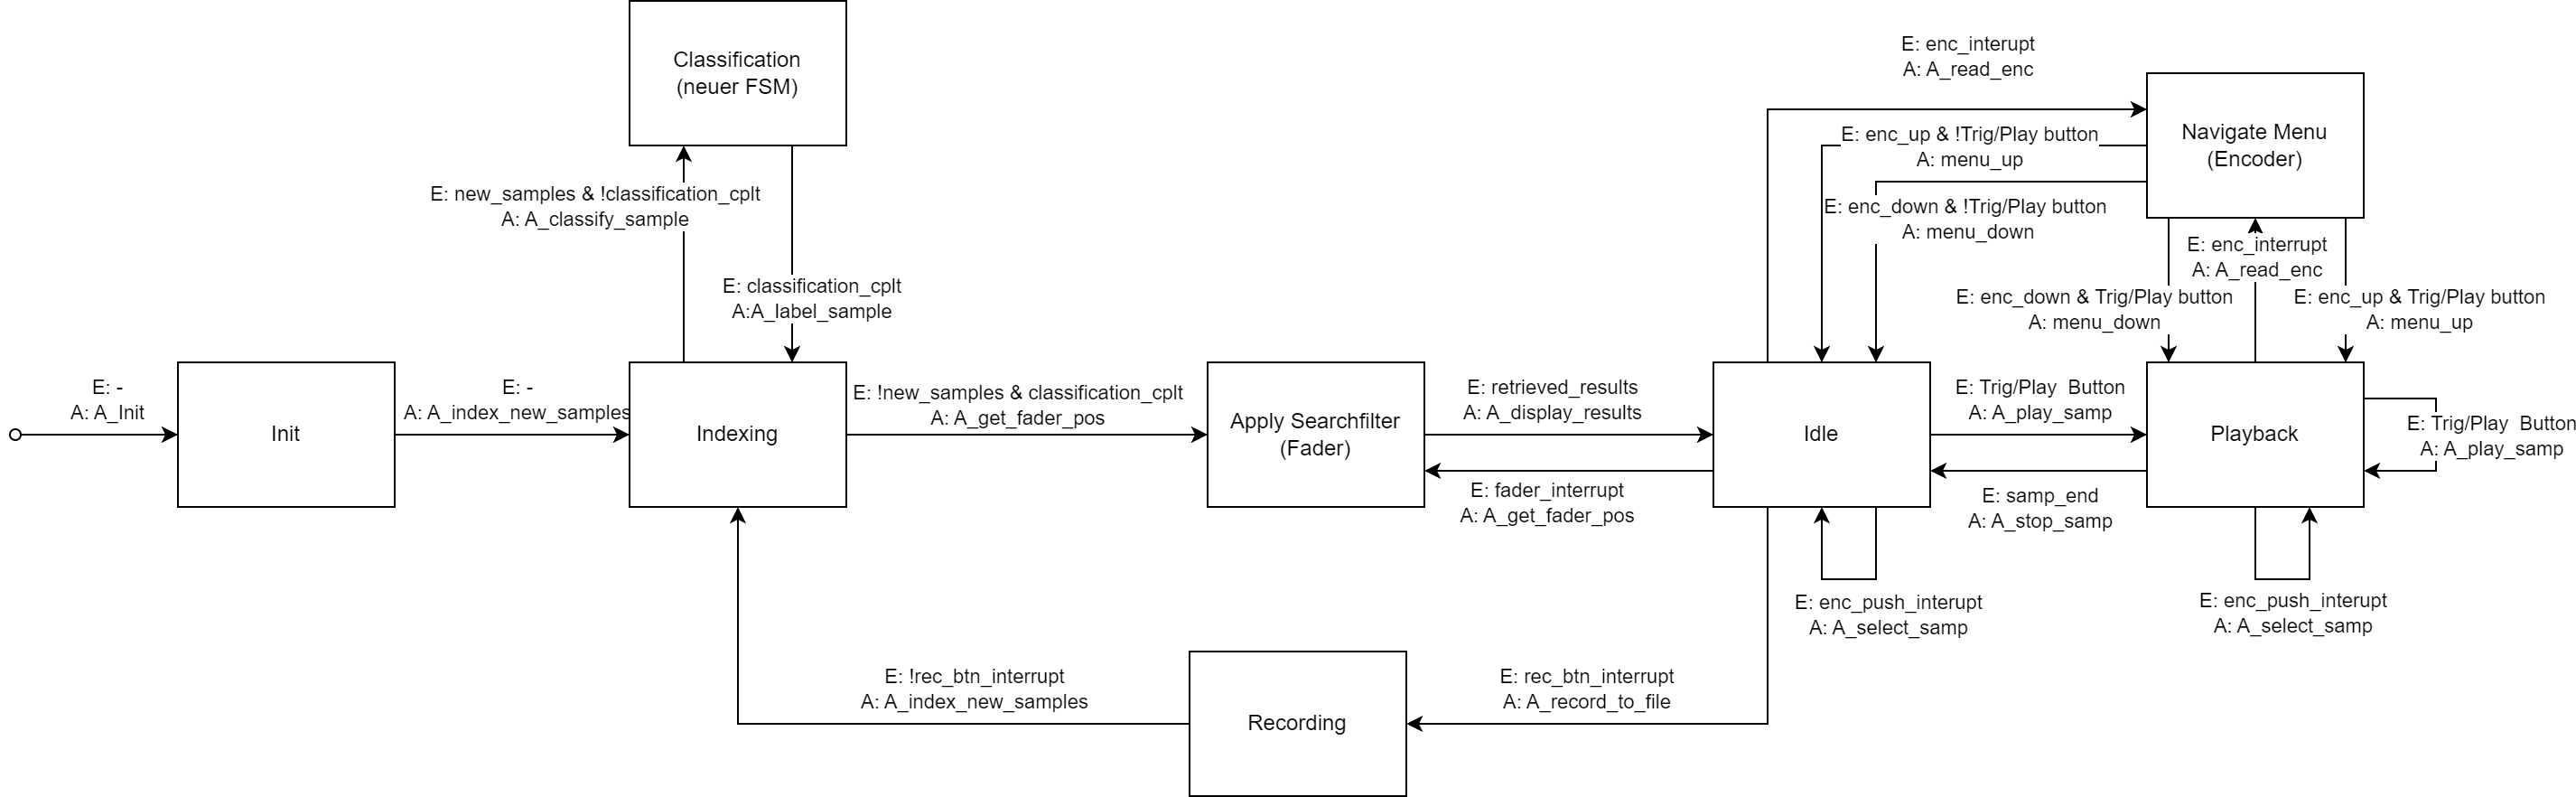
\includegraphics[width=1.0\textwidth]{images/04_spezifikation/fsm.drawio.png}
    	\caption{Zustandsautomat des Systems}
    	\label{fig:fsm}
    \end{figure}
    

\end{itemize}

\subsection{Arbeitspakete}

    \begin{figure}[H]
	\centering
	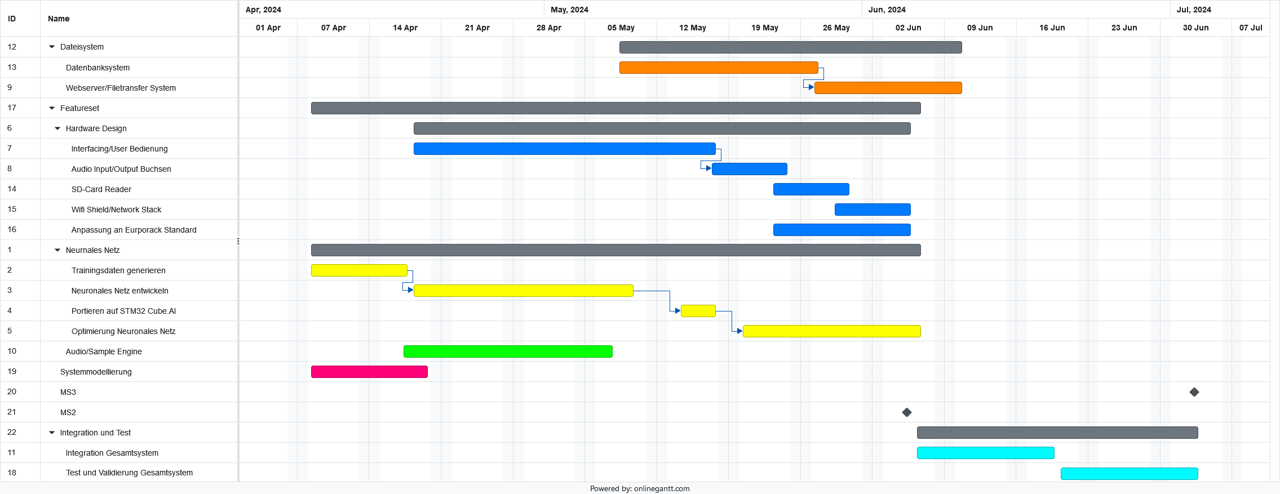
\includegraphics[width=1.0\textwidth]{images/04_spezifikation/gantt.png}
	\caption{GANTT Diagramm}
	\label{fig:gantt}
\end{figure}


Aufgabenaufteilung erläutern
\newpage

\subsection{Schnittstellenbeschreibung und Integration der Komponenten}
\begin{itemize}
    \item Planung der Schnittstellen zwischen den Komponenten
    \item Einfaches Diagramm in DrawIO:
    \begin{itemize}
        \item Zwischen Jonas und Leon: \texttt{downsampleandread1024()}
        \item Zwischen Syzmon und Jonas: \texttt{filemanager struct}, etc.
        \item Zwischen Szymon und Leon: \texttt{filemanager struct}
    \end{itemize}
    
    
    Folgendes Diagramm zeigt die Relation und Interaktion der 4 Komponenten miteinander.
    
    \begin{figure}[H]
    	\centering
    	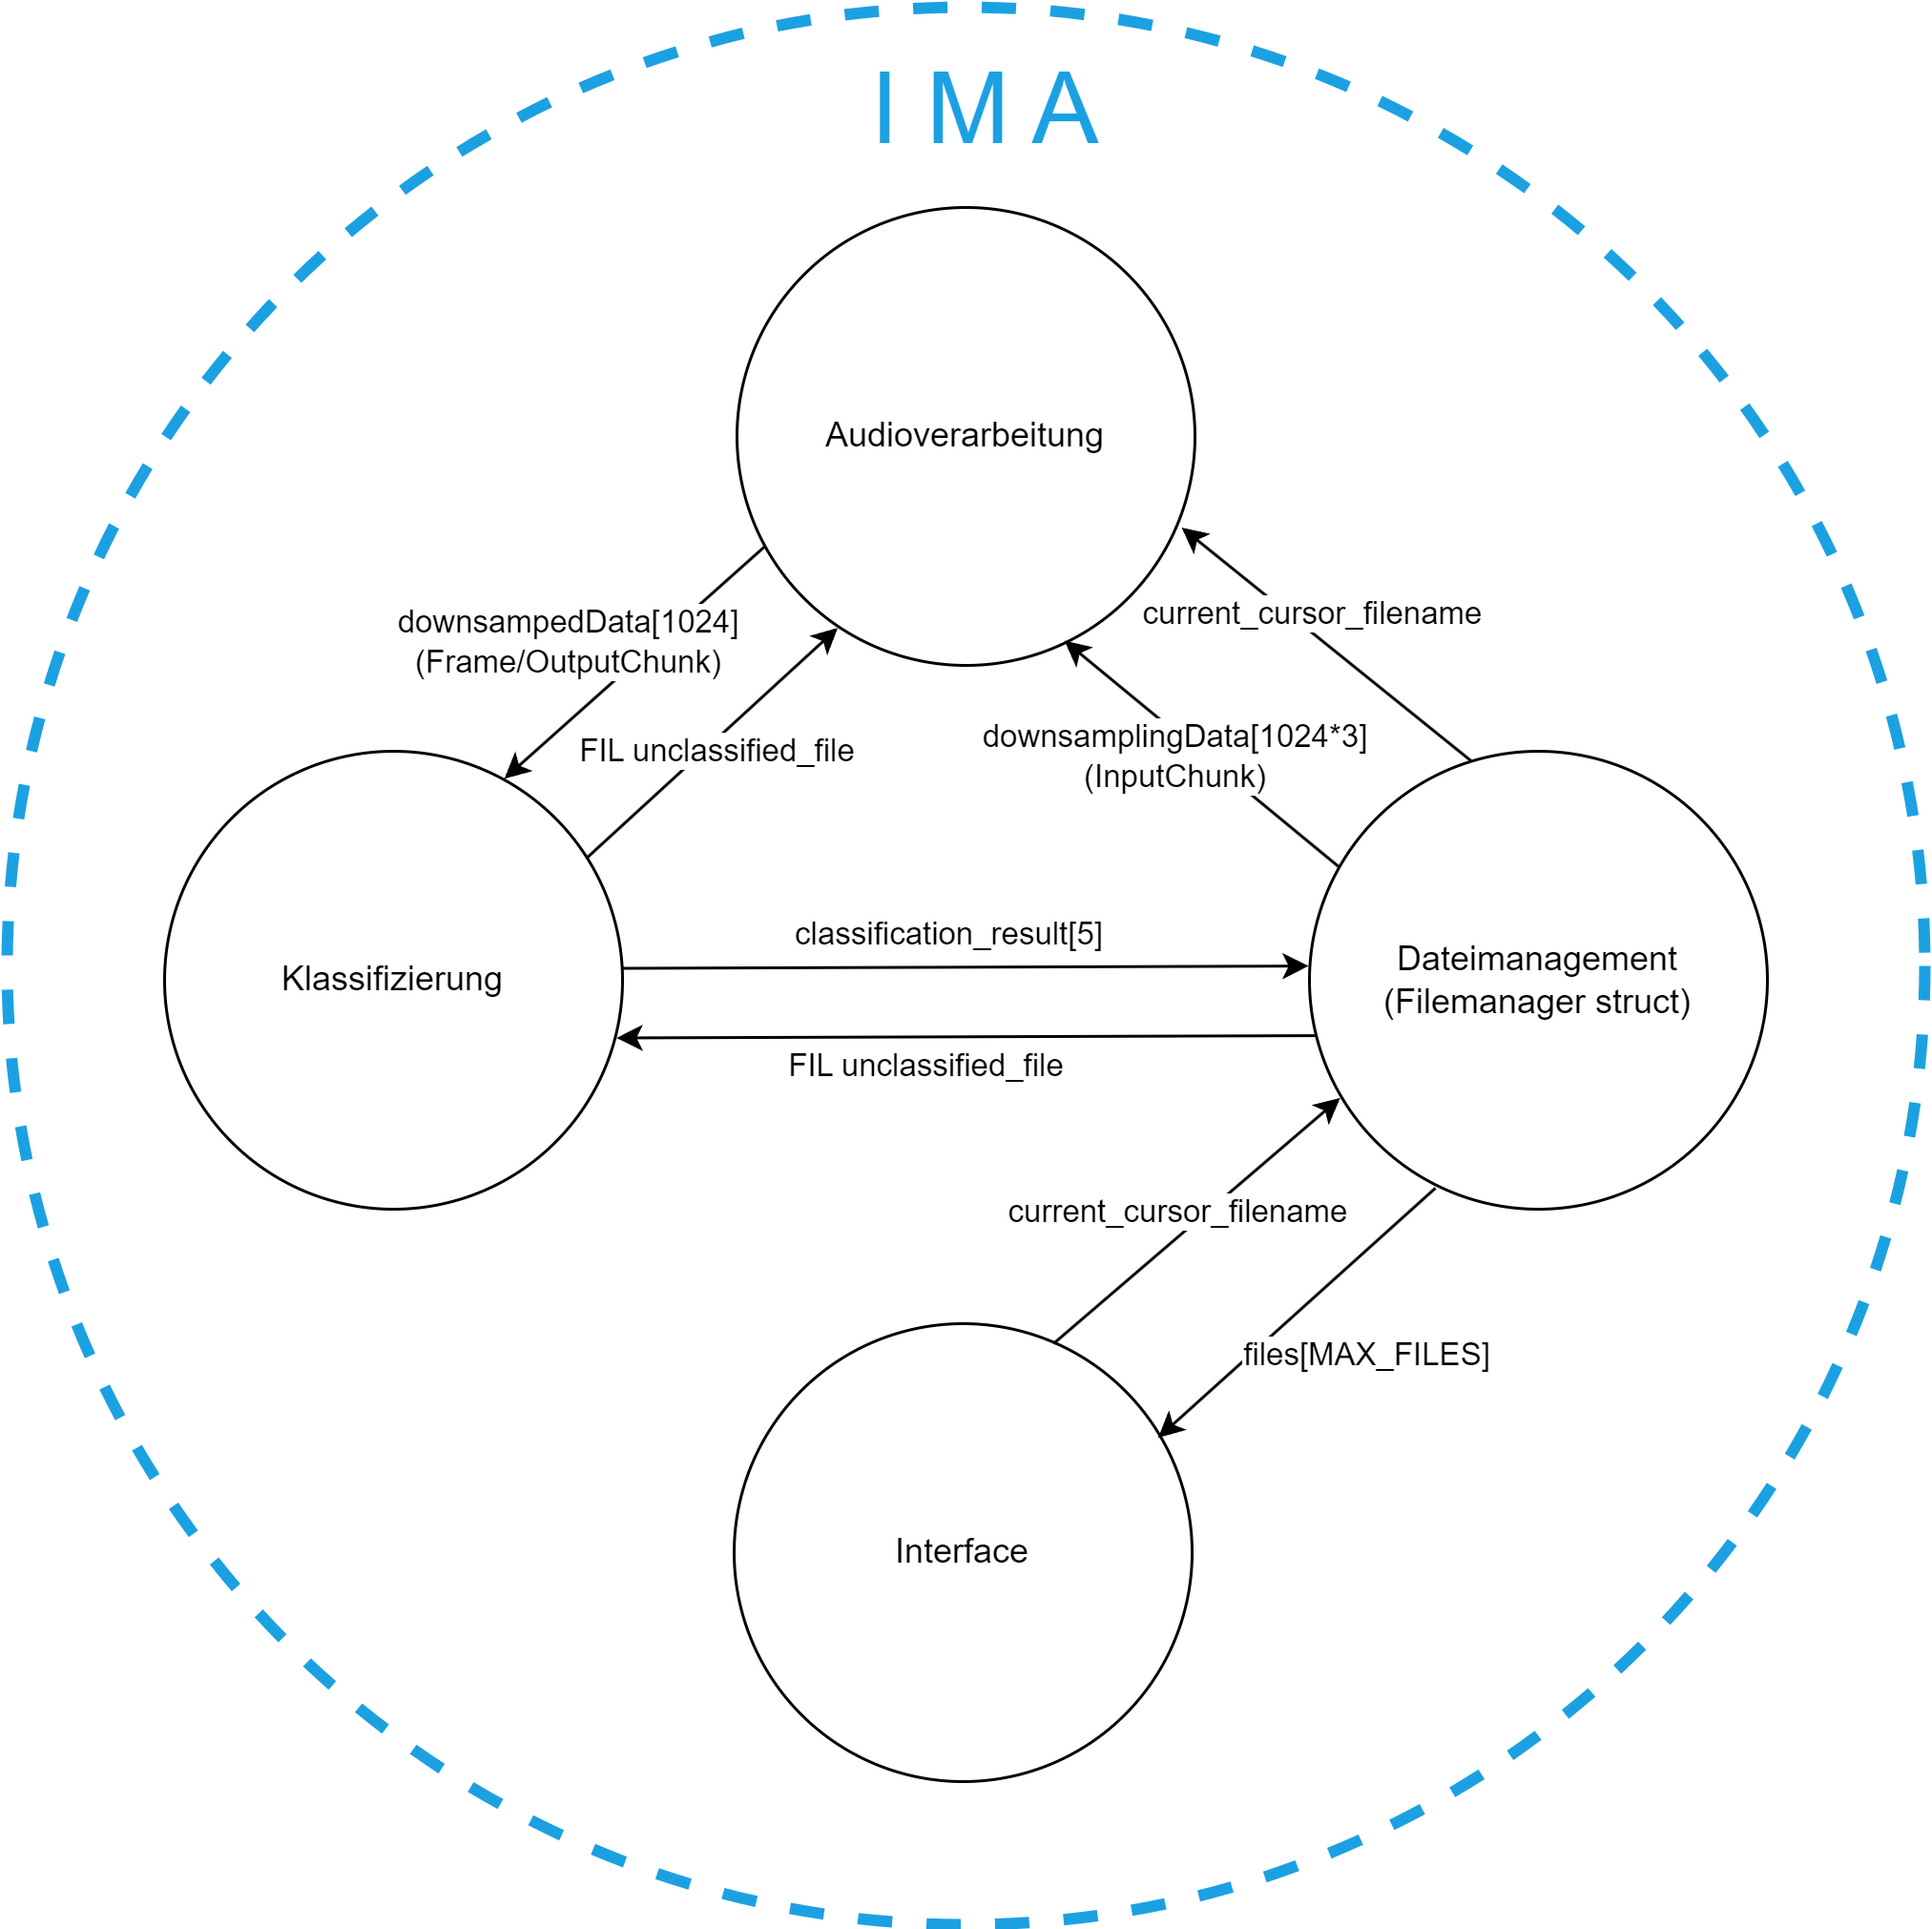
\includegraphics[width=1.0\textwidth]{images/04_spezifikation/komponentendiagramm.drawio.png}
    	\caption{Komponentendiagramm}
    	\label{fig:komponentendiagramm}
    \end{figure}
    
\end{itemize}

Das Dateimanagement ist der zentrale Knotenpunkt des Gesamtsystems. Es dient zunächst als Zugriffspunkt auf die Samples anhand ihrer Namen. 

Beim Hinzufügen neuer \textbf{Samples} in das Dateisystem werden diese zunächst als \boldinline{unclassified_file Fil} an die \boldinline{Klassifizierung} übergeben. Dieser wird an die Audioverarbeitung weiter gegeben. 
 
Diese gibt ein \boldinline{classification_result[5]} zurück, welcher den Dateien zugeordnet wird.


\newpage
\subsection{Technische Spezifikation}
Dieser Abschnitt behandelt die technischen Anforderungen des Projekts, die für die Umsetzung der verschiedenen Lastenfälle erforderlich sind. Es wird beschrieben, welche Hardware für jeden Lastenfall benötigt wird und aus welchen Gründen diese Auswahl getroffen wurde. Zudem wird die Wahl bestimmter Standards und Protokolle erläutert, die im Projekt verwendet werden.

\subsubsection{Hardware}


\textbf{Komponenten\hyperlink{LF01_Link}{/LF01/}} \\

\begin{wrapfigure}{r}{0.4\textwidth} % Increase the width of the figure environment
	\vspace{-60pt + 0.02\textwidth}
	\hspace{0.07\textwidth} % Add horizontal space
	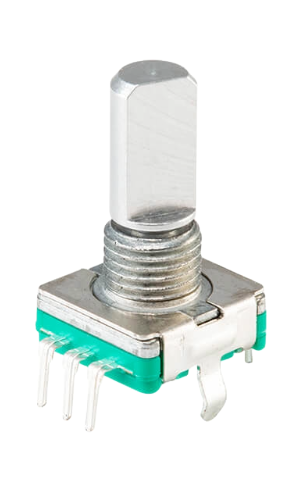
\includegraphics[width=0.2\textwidth]{images/05_technische_spezifikation/Interface/Encoder.png} % Keep the image size the same
	\caption{Rotary-Encoder}
	\label{fig:rotary_encoder}
	\vspace{-100pt}
\end{wrapfigure}

\textbf{\hypertarget{Encoder}{Encoder}} \\

\textbf{Model} RIC11-22S16D5M-TH

\textbf{Spannung} 3.3V

\textbf{Mechanisch:}
\begin{itemize}
	\item 20 Impulse pro Umdrehung (20 PPR)
	\item 20 Positionen (20 DET)
	\item Schalter (SW)
\end{itemize} 



Zur Auswahl der Samples und zum Navigieren durch das Menü wir ein Rotary-Encoder mit einem Switch Button eingesetzt.Das Empfangen der \textbf{A} und \textbf{B} Signale des Encoders erfolgt über die Pins \boldinline{PA0} und \boldinline{PA1}.
Das Drücken des Switch über den Pin \boldinline{PA4}. Durch das drücken des Switch-Buttons wird der Pin \boldinline{PA4} auf high gesetzt.

\begin{itemize}
	\item \textbf{Präzise Steuerung:} Der Encoder ermöglicht eine präzise Steuerung des Cursors auf dem Display.
	
	\item \textbf{Benutzerfreundlichkeit:} Der Benutzer kann durch die Liste navigieren und ein Sample auswählen. Die Kombination aus Drehbewegung und Druckknopf-Funktionalität macht den Encoder intuitiv.  
\end{itemize}

\vspace{3em}

\begin{wrapfigure}{r}{0.4\textwidth} % Increase the width of the figure environment
	\vspace{-20pt + 0.02\textwidth}
	\hspace{0.06\textwidth} % Add horizontal space
	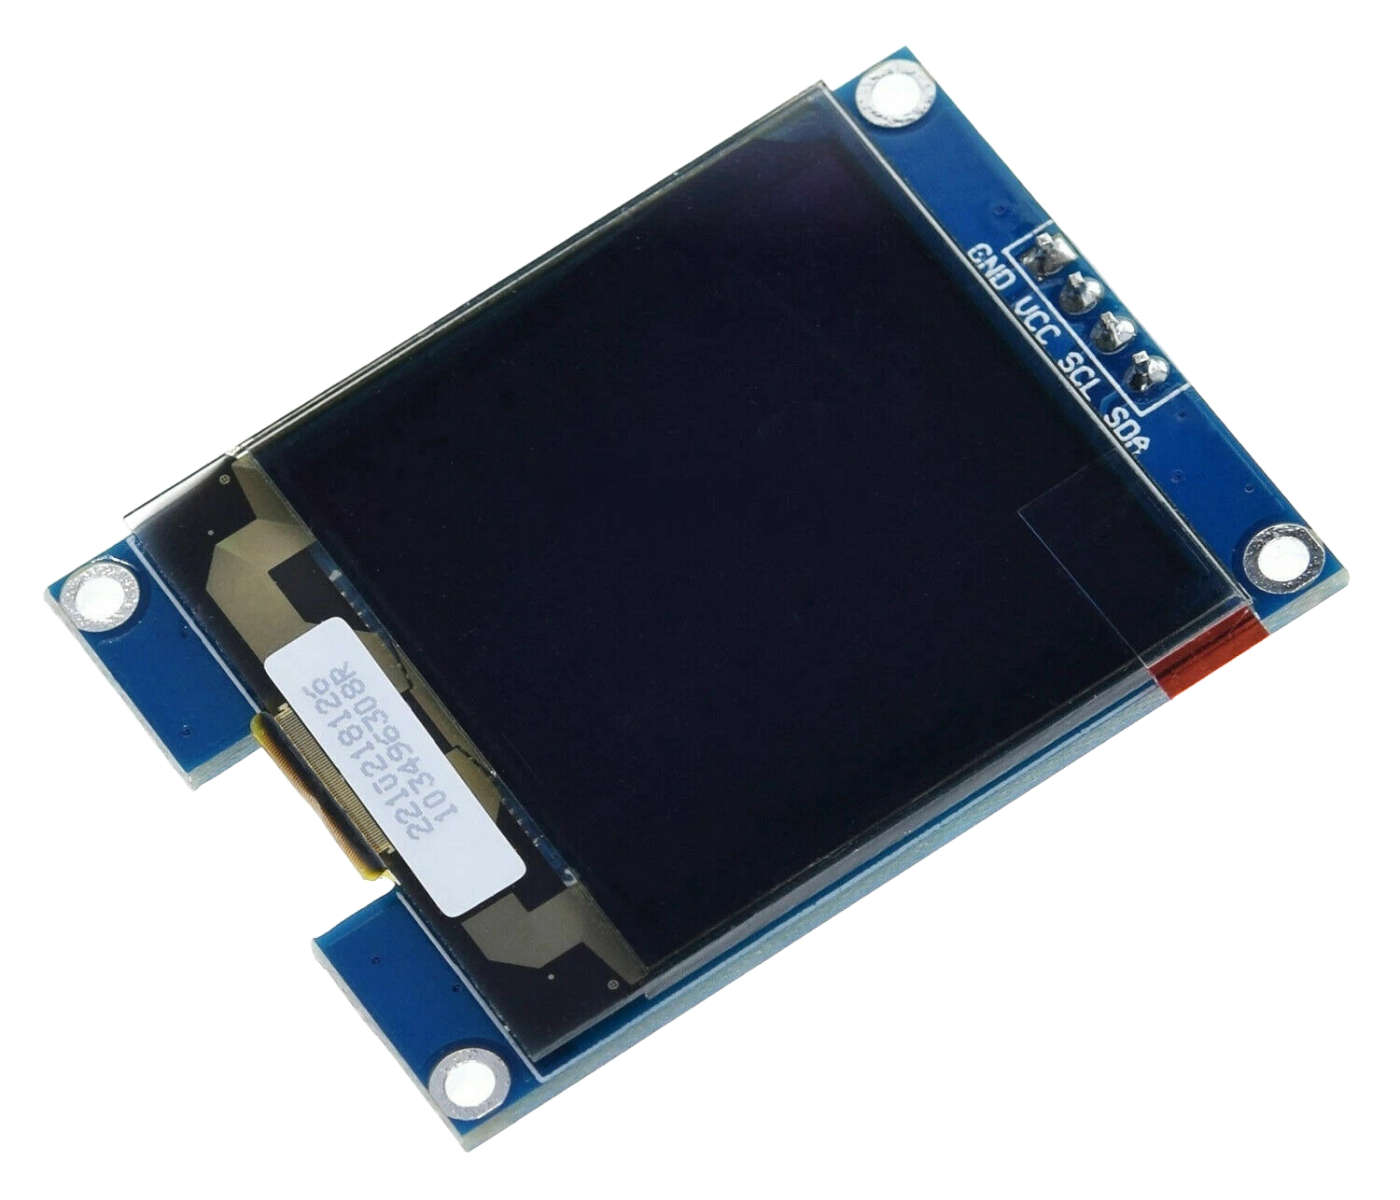
\includegraphics[width=0.25\textwidth]{images/05_technische_spezifikation/Interface/Display.png} % Keep the image size the same
	\caption{LCD-Display}
	\label{fig:lcd_display}
	\vspace{-50pt}
\end{wrapfigure}

\textbf{\hypertarget{Display}{LCD-Display}} \\

\textbf{Model:} GME128128-01-ii2

\textbf{Treiber:} SH1107

\textbf{Mode} Monochrom (1Bit)

\textbf{Spannung} 5.0V \\ \\



Zur Visualiesierung der Sampels haben wir einen Monochronen LCD-Display benutzt. Im zusammenspiel mit dem Encoder ermöglicht es eine gute Navigation durch den gewünschten Samplepool. Die Daten werden über den Output Pin  \boldinline{PB7} an den SDA des Displays übertragen. Der Takt wird über den Pin  \boldinline{PB6} an den SCL übertragen. Das Display wird mit 20 FPS betrieben und mit hilfe von \boldinline{Timer tim5} geupdated.

\begin{itemize}
	\item \textbf{Klare Visualisierung:} LCD-Displays bieten eine klare und gut lesbare Darstellung von Text und Grafiken.
	\item \textbf{Anpassbarkeit:} Sie können einfach an verschiedene Layouts und Designs angepasst werden.
\end{itemize}

\newpage
\textbf{Komponenten\hyperlink{LF02_Link}{/LF02/}} \\

\textbf{\hypertarget{Potentiometer}{Schiebe-Potentiometer}}\\

\textbf{Model} Bourns PTL45-15R0-103B2

\textbf{Wiederstand} 10k Ohm

\textbf{Weg} 45mm

\textbf{Spannung} 3.3V \\ \\ \\

	\begin{wrapfigure}{r}{0.4\textwidth} % Increase the width of the figure environment
	\vspace{-155pt + 0.02\textwidth}
	\hspace{0.07\textwidth} % Add horizontal space
	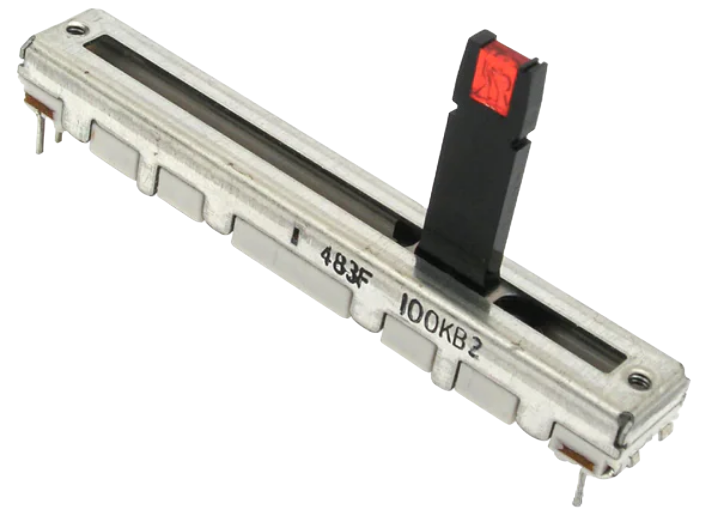
\includegraphics[width=0.2\textwidth]{images/05_technische_spezifikation/Interface/Potentiometer.png} % Keep the image size the same
	\caption{Potentiometer}
	\label{fig:schiebe_potentiometer}
	\vspace{-20pt}
\end{wrapfigure}

Für die Filterfunktion benötigen wir 5 Potentiometer. Es wird zyklisch die Ausgangsspannung des Schleifers abgegriffen die die Teilspannung zwichen den VCC und dem GND darstellt. Dies erfolgt mit Hilfe vom ADC und dem DMA. Die Auswertung der Spannung erfolgt über die Pins  \boldinline{PA6, PA7, PB0, PB1, PC0}. Die Pins  \boldinline{PA6, PA7, PB0, PB1} sind für die Klassen zuständig  \boldinline{PC0} für den Schwellenwert an erlaubter Abweichung.

\begin{itemize}
	\item \textbf{Präzise Steuerung und feine Abstimmung:} Ein Potentiometer ermöglicht eine stufenlose und präzise Einstellung. Durch das Schieben des Potentiometers kann der Benutzer den Cursor in kleinen, genauen Schritten bewegen.
	\item \textbf{Einfache Bedienung und intuitive Nutzung:} Potentiometer sind einfach und intuitiv zu bedienen.
	\item \textbf{Direkte visuelle Rückmeldung:} Durch die sofortige visuelle Rückmeldung auf dem LCD-Display kann der Benutzer sofort sehen, wie sich die Bewegung des Potentiometers auf die Position des Cursors auswirkt.
\end{itemize}


\textbf{(LCD-Display)}\\

Der LCD-Display ist der gleiche wie im \boldinline{/LF01/} beschrieben. Dieser dient zur Darstellung der Fader Einstellung in prozentualer Form.

\newpage

\subsubsection{Pinout Interface Komponente}

\textbf{Interface}

\begin{longtable}[c]{|p{2.5cm}|p{1cm}|p{2.5cm}|p{2.5cm}|p{2.5cm}|p{3cm}|}
	\hline
	\textbf{Komponente} & \textbf{PIN} & \textbf{Signal-On-PIN} &  \textbf{GPIO-Mode} & \textbf{GPIO-Pull-Up/Pull-Down } & \textbf{User-Label}\\
	\hline
	Encoder Menü & PA0 & n/a & EIMRETD & PULL UP & enc\_a\_clk\_in1 \\
	\hline
	& PA1 & n/a &  INPUT & PULL UP & enc\_a\_dt\_in2 \\
	\hline
	& PA4 & n/a & EIMRETD & PULL UP & enc\_a\_switch\_in3 \\
	\hline
	ADC & PA6 & ADC1\_IN6 & ANALOG & NPU NPD & FADER1 \\
	\hline
	& PA7 & ADC1\_IN7 & ANALOG & NPU NPD & FADER2 \\
	\hline
	& PB0 & ADC1\_IN8 & ANALOG & NPU NPD & FADER3 \\
	\hline
	& PB1 & ADC1\_IN9 & ANALOG & NPU NPD & FADER4 \\
	\hline
	& PC0 & ADC1\_IN10 & ANALOG & NPU NPD & FADER5 \\	
	\hline
	I2C & PB6 &I2C1\_SCL & AFOD & PULL UP & n/a \\
	\hline
	& PB7 &I2C1\_SDA & AFOD & PULL UP & n/a \\
	\hline
	SDIO & PC8 & SDIO\_D0 & AFPP & PULL UP & n/a \\
	\hline
	& PC9 & SDIO\_D1 & AFPP & PULL UP & n/a \\
	\hline
	& PC10 & SDIO\_D2 & AFPP & PULL UP & n/a \\
	\hline
	& PC11 & SDIO\_D3 & AFPP & PULL UP & n/a \\
	\hline
	& PC12 & SDIO\_CK & AFPP & NPU NPD & n/a \\
	\hline
	& PD2 & SDIO\_CMD & AFPP & PULL UP & n/a \\
	\hline
\end{longtable}

\textbf{EIMRETD} = External Interrupt Mode and Rising Edge Trigger Detection 		

\textbf{AFOD} = Alternate Function Open Drain

\textbf{NPU NPD} = No Pull Up No Pull Down		

\textbf{AFPP} = Alternate Function Push Pull


\newpage

\textbf{Komponenten\hyperlink{}{/LFxx/}} \\

\paragraph{PCM5102a Breakout Board}

\begin{wrapfigure}{r}{0.4\textwidth} % Increase the width of the figure environment
	\vspace{-20pt}
	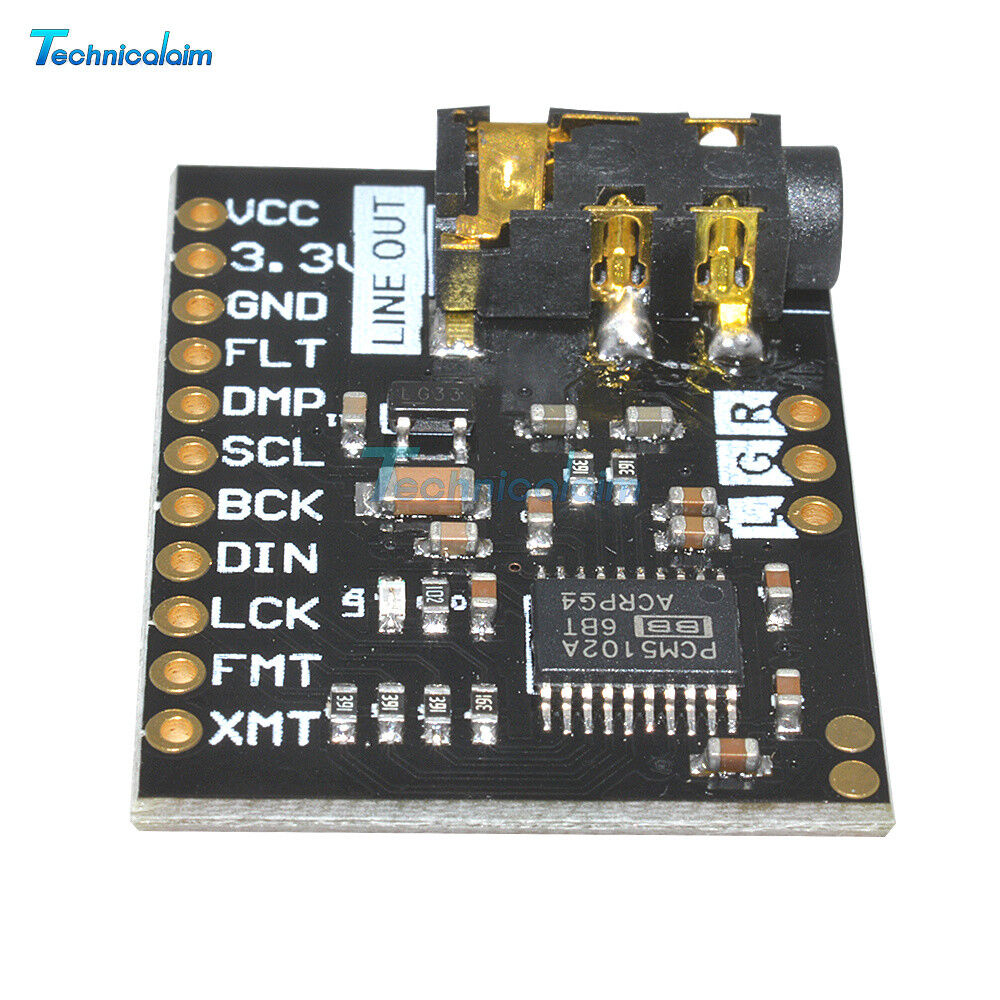
\includegraphics[width=0.2\textwidth]{images/05_technische_spezifikation/audio/pcm5102a_breakout.jpg}
	\caption{PCM5102a Breakout Board}
	\label{fig:pcm5102a_breakout}
\end{wrapfigure}

Der PCM5102a Audio Codec wurde für die DAC Wandlung der Audiodaten verwendet. Für die Implementation und die Entwicklung des Prototyps wurde ein Breakout Board gekauft, um ohne die Notwendikeit eines PCB-Design die Firmware für \textbf{I M A} zu schreiben. 
Komfortablerweise ist direkt eine \SI{3,5}{\milli\meter} Stereo-Klinkenbuchse auf dem Board verbaut.
Der Pegel beträgt Line-Level (\SI{\pm 1.7}{\volt_{rms}}), und ist somit grob kompatibel zum Eurorack-Standard.

Das Breakout Board wird mit einer Versorgungsspannung von \SI{3,3}{\volt} betrieben.

Als Übertragungsprotokoll dient \textbf{I2S}. Die detaillierte Inbetriebnahme findet sich in Abschnitt \ref{sec:pcm5102a-und-i2s}.


\paragraph{Waveshare Micro SD-Card Module}

\begin{wrapfigure}{r}{0.4\textwidth} % Increase the width of the figure environment
	\vspace{-20pt}
	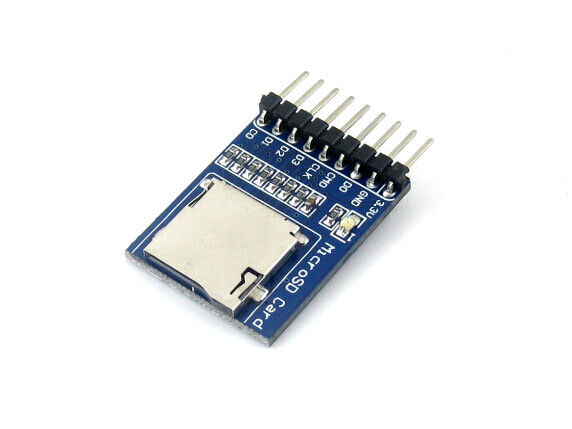
\includegraphics[width=0.4\textwidth]{images/05_technische_spezifikation/audio/waveshare_micro_sd_module.jpg}
	\caption{Waveshare Micro SD-Karten Modul}
	\label{fig:waveshare_micro_sd_module}
\end{wrapfigure}

Das Waveshare Micro SD-Card Module wird für die Speicherung und den Zugriff auf Audiodaten in diesem Projekt verwendet. Dieses Modul ermöglicht die einfache Integration von Micro SD-Karten in das System, um persistente Daten zu lesen und zu schreiben, ohne aufwändige PCB-Designs oder zusätzliche Hardwarekomponenten implementieren zu müssen.

Das Modul unterstützt den Standard \textbf{SDIO}-Bus zur Datenübertragung, was eine einfache Anbindung an das Mikrocontroller-System ermöglicht. 

Die Inbetriebnahme und die spezifischen Konfigurationen für die Verwendung dieses Moduls werden in Abschnitt \ref{sec:sd-card-audio} detailliert beschrieben. 

Das Modul wird mit einer Versorgungsspannung von \SI{3.3}{\volt} betrieben.

\newpage
\subsubsection{Pinout Audio Komponente}

\textbf{Audio}
\begin{longtable}[c]{|p{2.5cm}|p{1cm}|p{2.5cm}|p{2.5cm}|p{2.5cm}|p{3cm}|}
	\hline
	\textbf{Komponente} & \textbf{PIN} & \textbf{Signal-On-PIN} &  \textbf{GPIO-Mode} & \textbf{GPIO-Pull-Up/Pull-Down } & \textbf{User-Label}\\
	\hline
	SDIO & PC8 & SDIO\_D0 & AFPP & PULL UP & n/a \\
	\hline
	& PC9 & SDIO\_D1 & AFPP & PULL UP & n/a \\
	\hline
	& PC10 & SDIO\_D2 & AFPP & PULL UP & n/a \\
	\hline
	& PC11 & SDIO\_D3 & AFPP & PULL UP & n/a \\
	\hline
	& PC12 & SDIO\_CK & AFPP & NPU NPD & n/a \\
	\hline
	& PD2 & SDIO\_CMD & AFPP & PULL UP & n/a \\
	\hline
	I2S & PB10 & IS2\_CK & AFPP  & NPU NPD & n/a \\
	\hline
	& PB12 & IS2\_WS & AFPP & NPU NPD & n/a \\
	\hline
	& PC3 & IS2\_SD & AFPP & NPU NPD &  n/a \\
	\hline
	& PC6 & IS2\_MCK & AFPP & NPU NPD &  n/a \\
	\hline
\end{longtable}

\textbf{NPU NPD} = No Pull Up No Pull Down		

\textbf{AFPP} = Alternate Function Push Pull 




\newpage
\subsubsection{Schaltpläne}
\label{sec:test-schematics}

% Including the first landscape schematic PDF as a single page with label

\begin{figure}[ht]
	\centering
	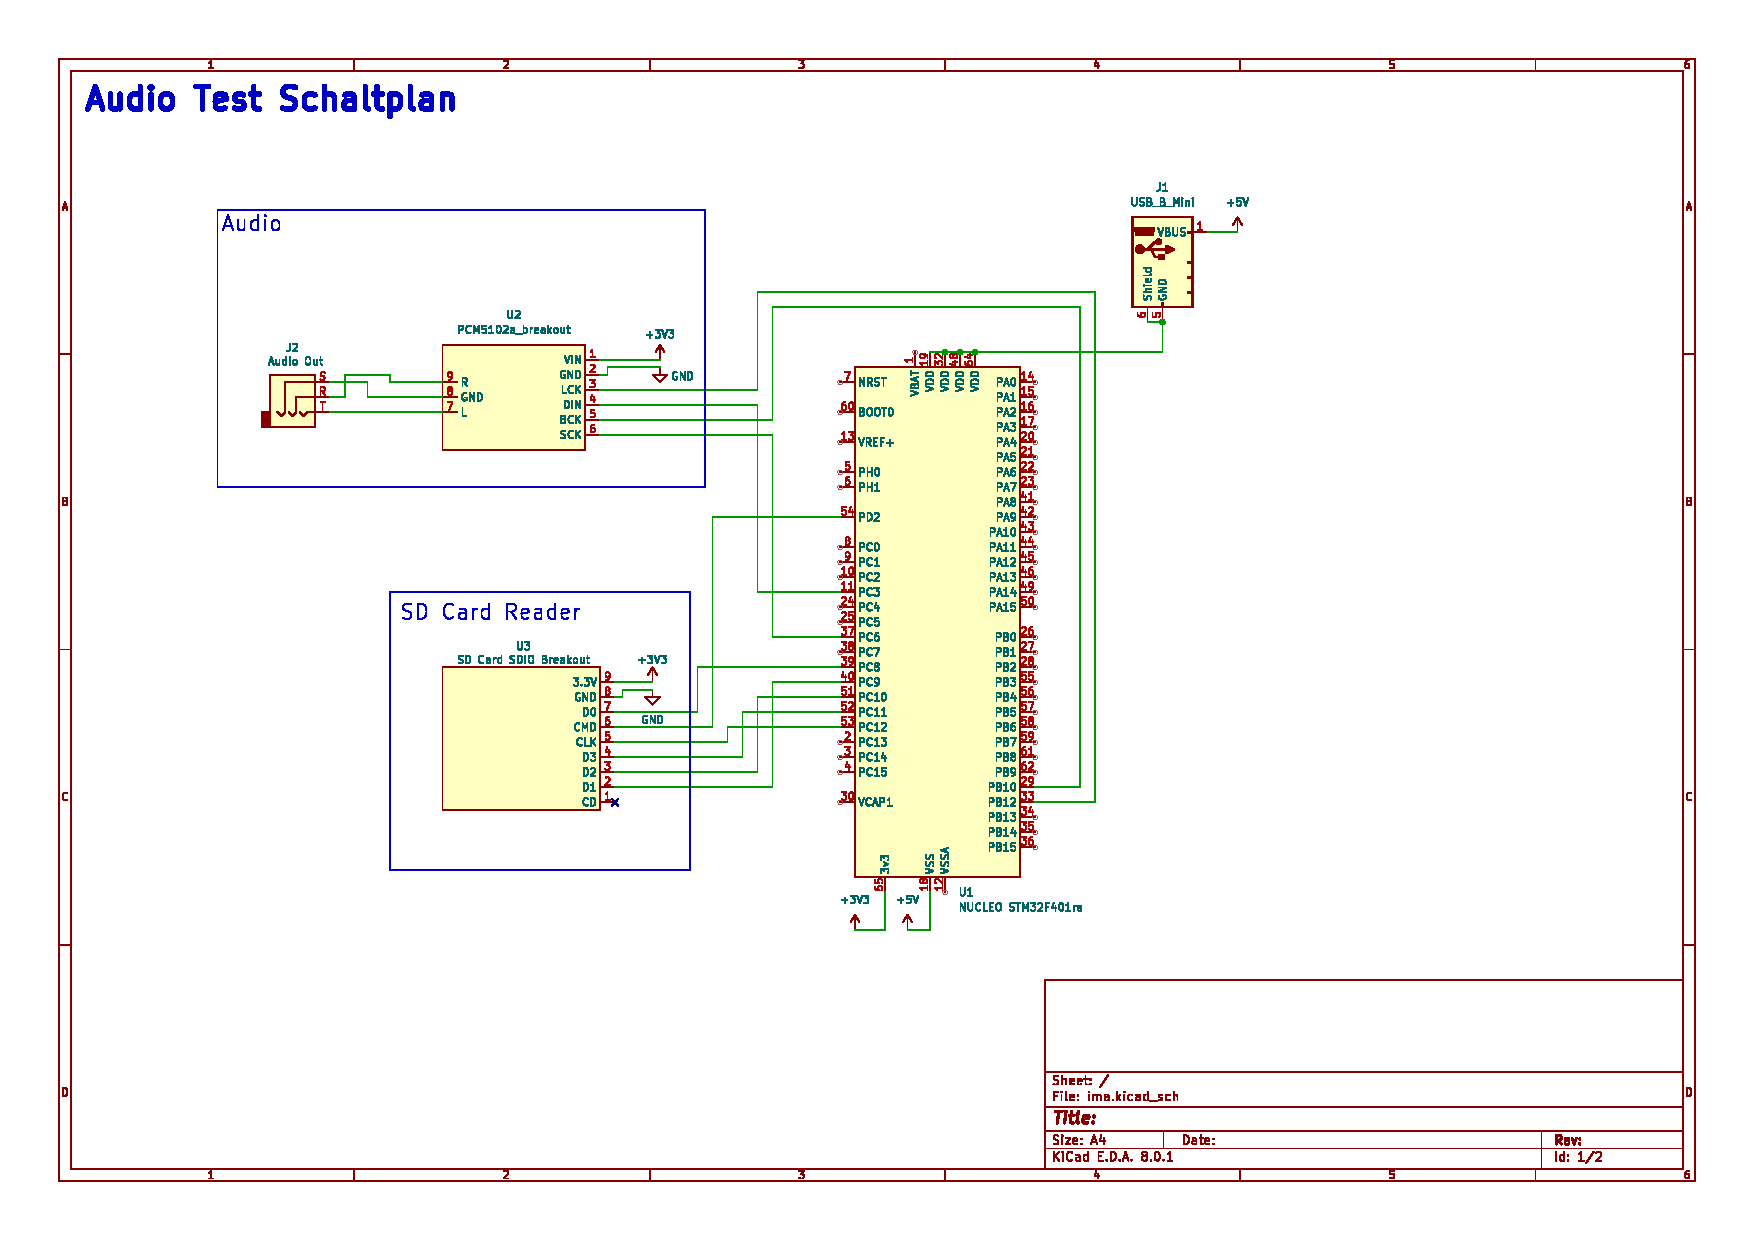
\includepdf[pages=-]{../schematics/audio_test_schematic.pdf}
	\label{fig:audio_test_schematic}
\end{figure}

\newpage
\begin{figure}[ht]
	\centering
	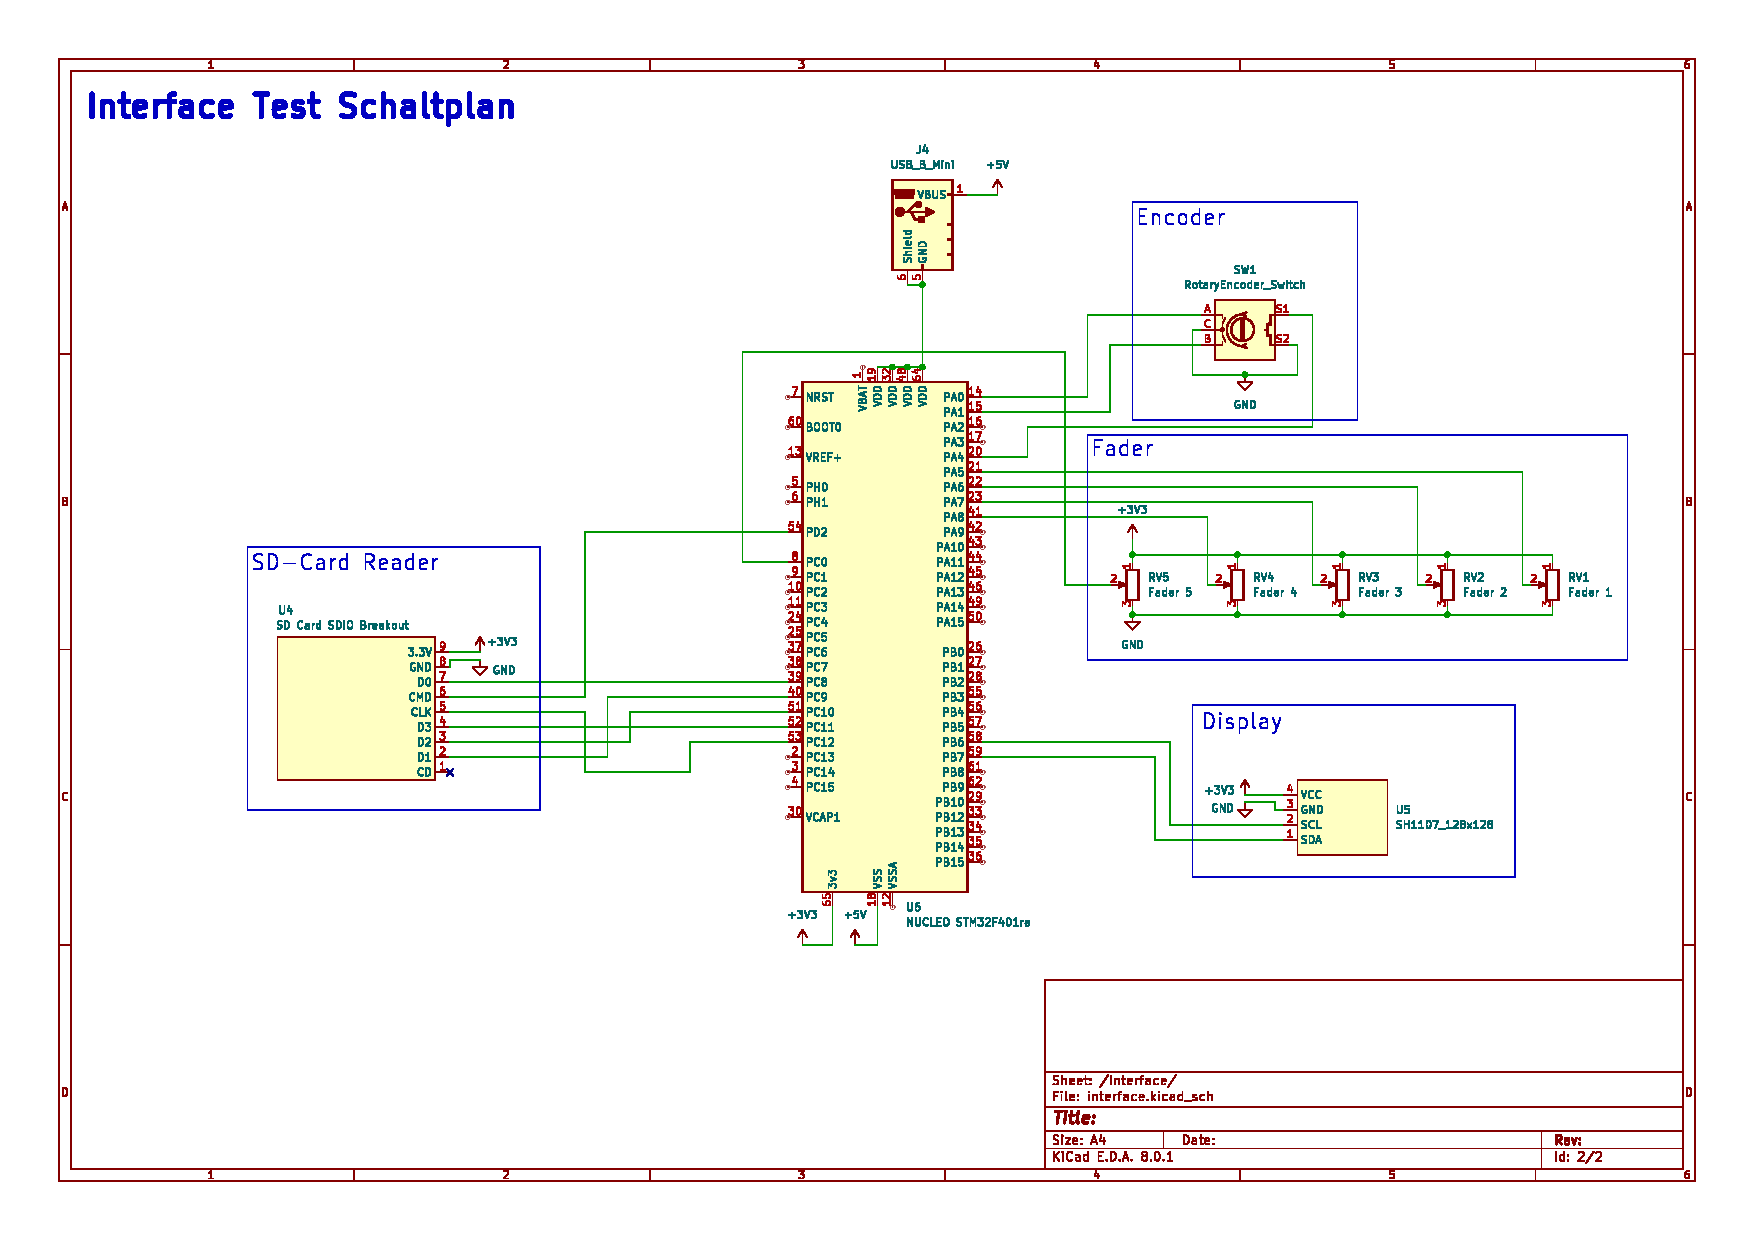
\includepdf[pages=-]{../schematics/interface_test_schematic.pdf}
	\label{fig:interface_test_schematic}
\end{figure}
\newpage
\section{Durchführung}

\subsection{Klassifizierung von Audiodateien durch ein Neuronales Netz}
Durch das neuronale Netz sollen digitale Audiodateien (Audiosamples) mit variabler Länge in fünf Merkmalsklassen klassifiziert werden. Dabei kann ein Datenpunkt, also ein Audiosample, mehreren Merkmalsklassen zugehörig sein. Dies wird als ``Multi-Label-Klassifizierung`` bezeichnet \cite{multilabel-classification}. Wird eine Audiodatei (Eingabevektor) zur Klassifizierung in das neuronale Netz eingegeben, erhält man als Ausgabe einen Ausgabevektor von fünf Werten zwischen 0.00 und 1.00, wobei jeder der fünf Werte  die Ähnlichkeit mit einer der fünf Merkmalsklassen repräsentiert (0.00 $\equiv$ keine Ähnlichkeit, 1.00 $\equiv$ Übereinstimmung). Die Merkmalsklassen werden wie folgt definiert:
    \begin{itemize}
        \item \textbf{bass:} Das Audiosample enthält Töne aus dem tiefen Frequenzspektrum
       	\item \textbf{pitched:} Das Audiosample enthält Töne aus dem hohen Frequenzspektrum
        \item \textbf{melodic:} Das Audiosample enthält melodische Elemente
        \item \textbf{rhythmic:} Das Audiosample enthält rhytmische Elemente
        \item \textbf{sustained:} Das Audiosample enthält ``flächige`` Elemente, also ``langgezogene`` Töne
    \end{itemize}

Dieses neuronale Netz wird mit selbst generierten Trainingsdaten trainiert und anschließend als fertiges Modell mittels dem STM32 proprietären Tool ``STM32Cube.AI`` in C-Code umgewandelt. Damit kann das Neuronale Netz im eigenen Code als normale C-Funktion verwendet werden, mit dem Eingabevektor (Audiodaten) als Funktionsparameter und dem Ausgabevektor (Klassifikationsergebnis) als Rückgabewert. \cite{stm32-cube-ai-documentation}

\begin{wrapfigure}{r}{0.4\textwidth}
    \centering
    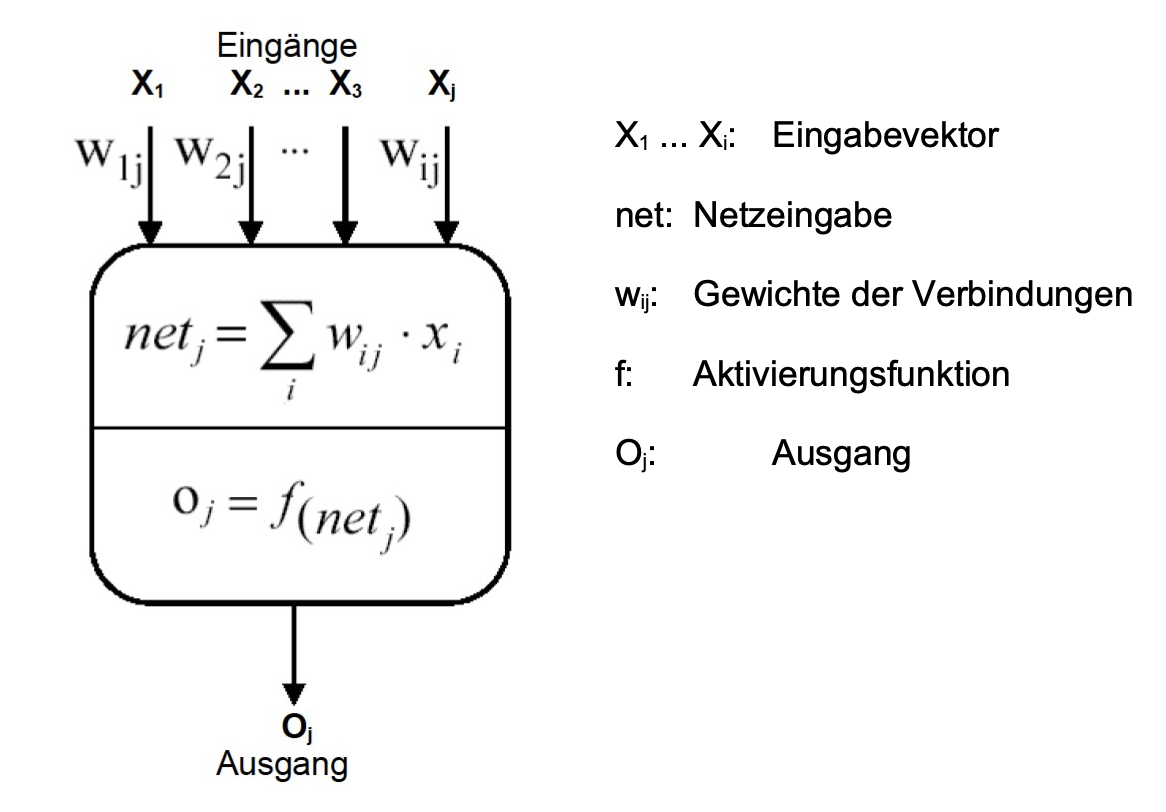
\includegraphics[width=0.4\textwidth]{images/08_durchfuehrung/neuron-aufbau.png}
    \caption{Aufbau des künstlichen Neurons. Quelle: Thieling, Lothar: “Neuronale Netze (Vorlesungsskript ML)”, Kapitel F, Seite 6.}
    \label{fig:img-aufbau-neuron}
\end{wrapfigure}

Die Umwandlung in C-Code ist mögich, da ein künstliches Neuron, wie in \textbf{\autoref{fig:img-aufbau-neuron}} dargestellt, aus aus mehreren Gewichten (\textit{W\textsubscript{x}}) in Form eines Vektors besteht, der mit dem Eingabevektor (\textit{X\textsubscript{n}}) des Neurons multipliziert wird. Beide Vektoren sind Fließkommazahlen. Anschließend werden diese Produkte aufaddiert und als Eingabewert einer mathematischen Funktion, der sog. ``Aktivierungsfunktion`` (\textit{f}) verwendet. Der Ausgabewert dieser Funktion ist die Ausgabe des Neurons. \cite{neural-network-basics}

Bei einem neuronalen Netz werden die Neuronen in Schichten hinterheinander angeordnet, die Neuronen der benachbarten Schichten werden vereinfacht gesagt miteinander verbunden, also die Eingabe des einen Neurons bildet eine der Eingaben des nachfolgenden Neurons. \cite{neural-network-basics}

Sowohl die Multiplikation von Vektoren, als auch die Berechnung von Funktionswerten ist in der Programmiersprache C problemlos möglich.

Der ressourcenintensive Teil des Umgangs mit neuronalen Netzen ist das Training, also der Anpassung der Gewichtswerte bis das Neuronale Netz akzeptable Ausgabewerte liefert \cite{neural-network-basics}. Bei diesem Prozess müssen vergleichsweise sehr viele Berechnungen durchgeführt werden. Aus diesem Grund wird das Neuronale Netz zuerst trainiert und erst dann als fertiges Modell in C-Code ungewandelt und auf dem STM32 Microcontroller betrieben. 
Dass das Neuronale Netz fortlaufend durch Benutzerinteraktion weiter trainiert wird, ist nicht vorgesehen.


\subsubsection{Ansatz für die Klassizierung von Audiodaten}
\label{sec:approach-audio-classification}
Die Audiosamples liegen als WAVE-Dateien (Dateiendung .wav) vor. Diese enthalten in der Regel pulsweitenmodulierte (PCM) Audiodaten \cite{wav-contains-pcm-data}. Da die Daten nicht komprimiert sind, gehören sie in der Audio- und Musikindustrie zu den gängigsten Dateiformaten \cite{wav-popular-file-format-music-industry}. Eine typische Samplerate für WAVE-Dateien beträgt 44,1 kHz, also 44.100 Samples pro Sekunde, wobei ein Sample in der WAVE-Datei ein quantisierter Amplitudenwert zu einem bestimmten Zeitpunkt ist \cite{wav-pcm-data}. Plottet man dies als Graph, könnte ein Audiosignal wie in \textbf{\autoref{fig:img-pcm-graph}} aussehen.


\begin{figure}[h!]
\centering
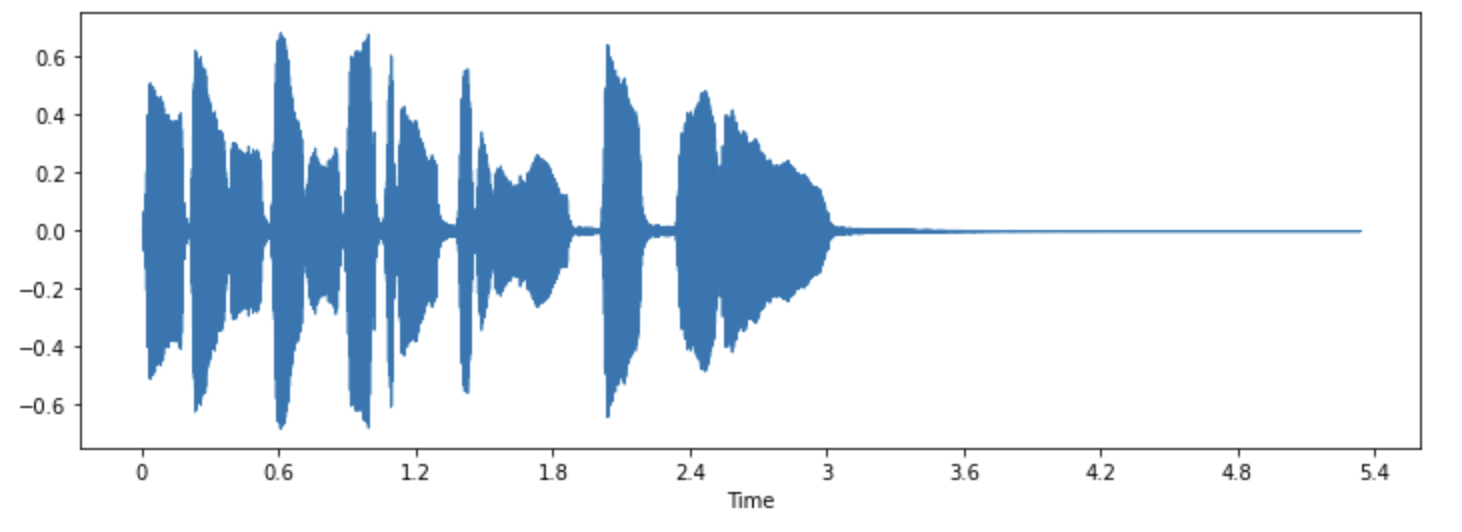
\includegraphics[width=0.6\textwidth]{images/08_durchfuehrung/waveform_plot.png}
\caption{Darstellung eines PCM Audiosignals, Quelle:  https://huggingface.co/learn/audio-course/chapter1/audio\_data TODO }
\label{fig:img-pcm-graph}
\end{figure}

Diese Daten direkt durch ein neuronales Netz klassifizieren zu lassen, ist aus verschiedenen Gründen wenig praktikabel. Die zwei Hauptgründe sind die Merkmalsextraktion und die Größe des Eingabevektors. Letzterer Punkt würde dazu führen, dass selbst bei einer geringeren Samplerate von 16 kHz der Eingabevektor 16.000 Werte umfasst. Ein Downsampling auf eine deutlich geringere Zahl, z.B. 1000, ist aufgrund des Shannon-Nyquist-Theorems nicht praktikabel, da dieses besagt, dass die Samplerate mindestens doppelt so hoch sein muss wie die höchste Frequenz \cite{nyquist}. Damit läge der klassifizierbare Frequenzbereich nur im Bereich von \textit{0 Hz} bis maximal \textit{1000 / 2 = 500 Hz}.

Deutlich geeigneter ist es, die Daten als Spektrogramm (Amplitude der verschiedenen Frequenzen eines Signals über die Zeit) wie in \textbf{\autoref{fig:img-spectrogram}} darzustellen und mit einem Convolutional Neural Network (CNN) zu klassifizieren. CNNs werden in erster Linie zur Klassifizierung von Bildern eingesetzt. Die wesentliche Idee ist, dass das neuronale Netz dann nicht nur klassifiziert, sondern auch die Bildvorverarbeitung und die Merkmalsextraktion übernimmt \cite{how-cnn-work}. Da die Audiodateien für das menschliche Gehör klassifiziert werden, sind Mel-Spektrogramme besonders geeignet. Sie basieren auf der Mel-Skala, die das menschliche Gehör nachahmt. Die Mel-Skala ist eine nichtlineare Skala der Frequenzen, die mehr Gewicht auf tiefere Frequenzen legt \cite{mel-spectrogram}.

\begin{figure}[h!]
\centering
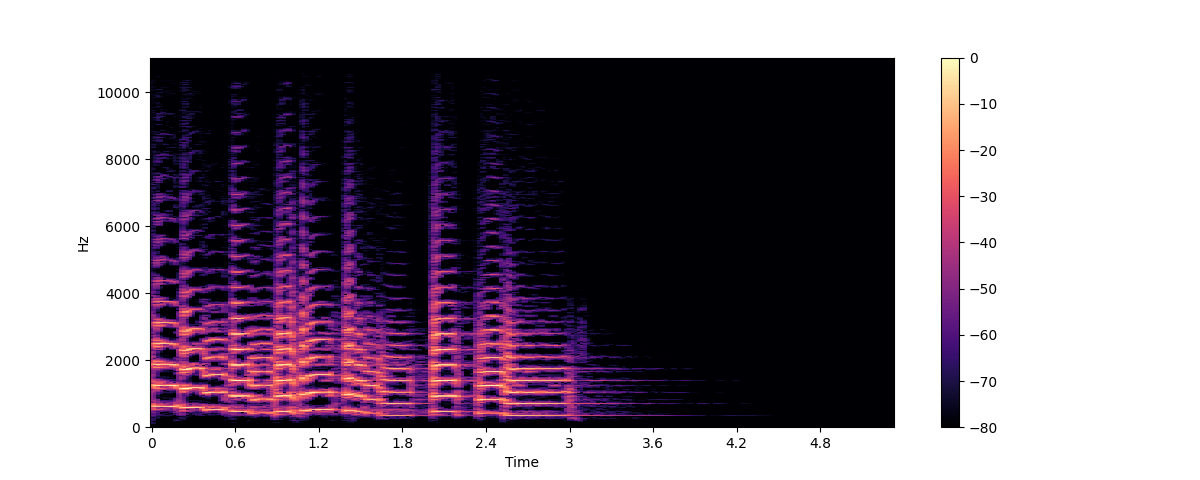
\includegraphics[width=0.75\textwidth]{images/08_durchfuehrung/spectrogram_plot.png}
\caption{Darstellung eines Audiosignals als Spektrogramm, Quelle:  https://huggingface.co/learn/audio-course/chapter1/audio\_data TODO }
\label{fig:img-spectrogram}
\end{figure}

Der limitierende Faktor beim Einsatz eines CNN auf einem Microcontroller sind die Hardwareressourcen, also in erster Linie Flash-Speicher und RAM.

Aufgrund der fehlenden Erfahrungswerte der Teammitglieder mit der möglichen Komplexität von neuronalen Netzen, die mit den Hardwareressourcen eines Microcontrollers betrieben werden können, wird sich auf ein Beispielprojekt von STMicroelectornics gestützt. Dieses heißt ``Acoustic Scene Classification`` \cite{stm-asc}\cite{stm-asc-2}. Kern ist die Klassifizierung von 30x32 px großen Mel-Spektrogrammen mit einem zwei Schichten CNN, die einen Eingabevektor von \textit{32 x 30 = 960} Werten ergeben. 

Sowohl die Dimensionierung der Spektrogramme, als auch die Topologie des Neuronalen Netzes, die Anzahl der Neuronen je Schicht und Elemente der Datenvorverarbeitung wurden aus diesem Projekt übernommen. Damit ist sicher gestellt, dass das Neuronale Netz am Ende nicht die Ressourcen des Microcontrollers übersteigt.

\subsubsection{Generieren der Eingabedaten}
\label{sec:input-data-generation}
Für das Training des neuronalen Netzes sind Trainingsdaten erforderlich. Diese bestehen aus Eingabedaten, die bereits mit den korrekten Klassifikationsergebnissen, also Labels, versehen sind. Um das Training des neuronalen Netzes während des Trainings einschätzen und nach Abschluss des Trainings validieren zu können, werden die Eingabedaten in drei Segmente aufgeteilt.

Da online keine kostenlosen und bereits mit den passenden Labels versehene Datensätze gefunden werden konnten, wurden eigene Daten generiert. Grundlage hierfür bildet eine private Audiosample-Bibliothek. Ein eigens entwickeltes Python-Skript ermöglicht es, Audiosamples auszuwählen, abzuspielen und zeiteffizient zu labeln.

Für jedes manuell gelabelte Audiosample wird eine eindeutige Identifikationsnummer (UID) generiert. Die zugehörigen Labels werden in einer CSV-Datei gespeichert. Ein Beispiel für einen solchen Datensatz zeigt \textbf{\autoref{tab:audiodaten}}. Außerdem wird eine Kopie des Audiosamples unter dem Namen der UID im Ausgabeordner des Skripts abgelegt. Diese Dateien werden später vom Jupyter-Notebook für das Training verwendet.

\begin{table}[h!]
\centering
\begin{tabular}{|m{2.8cm}|m{4.5cm}|m{0.8cm}|m{1.2cm}|m{1.5cm}|m{1.5cm}|m{1.3cm}|}
\hline
\textbf{UID} & \textbf{File} & \textbf{bass} & \textbf{pitched} & \textbf{sustained} & \textbf{rhythmic} & \textbf{melodic} \\ \hline
ecfad96b740844c3
9c96127279f22cf6 &  BD 606 Long MPC60 01.wav & 1 & 0 & 0 & 1 & 0 \\ \hline
\end{tabular}
\caption{Beispielhafter Datensatz eines Audiosamples}
\label{tab:audiodaten}
\end{table}

Bei der Auswahl der Audiosamples wurde darauf geachtet, dass die Daten annähernd gleich verteilt sind, um eine ausgewogene Trainingsbasis zu schaffen. Ein Ungleichgewicht in den Daten kann sich negativ auf das Training und die Klassifikationsergebnisse auswirken. Überrepräsentierte Merkmale könnten die Klassifikationsschwellenwerte beeinflussen, sodass die häufiger vorkommenden Klassen später bevorzugt erkannt werden. Wie in \textbf{\autoref{tab:img-class-spread-graph}} zu sehen, ist die Gleichverteilung jedoch zugegebenermaßen nur mäßig gelungen und hätte einen größeren Zeitaufwand erfordert.

\begin{figure}[h!]
\centering
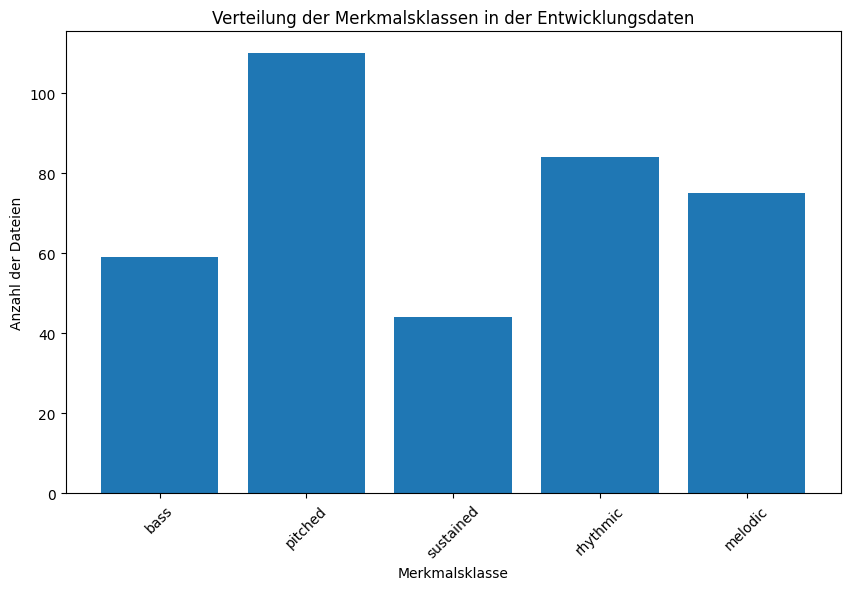
\includegraphics[width=0.75\textwidth]{images/08_durchfuehrung/class_spread_plot.png}
\caption{Repräsentation der verschiedenen Merkmalsklassen in den Entwicklungsdaten}
\label{fig:img-class-spread-graph}
\end{figure}

Zudem wurde sichergestellt, dass der Variationsbereich jeder Klasse möglichst umfassend abgedeckt ist. Dies umfasst sowohl reine Formen jeder Klasse – beispielsweise bei „pitched“ Audiosamples ausschließlich mit Tönen aus dem hohen Frequenzbereich – als auch Mischformen, die Merkmale mehrerer Klassen kombinieren.

Insgesamt wurden 207 Audiosamples unterschiedlicher Länge mit Labels versehen.

Insgesamt wu
TODO:

- wie viele Eingabe-Audiosamples

- wie viele Trainingsdatensätze

- Aufteilung der Daten (Grafik)

- Quellen

\subsubsection{Datenvorverarbeitung}

Für die Datenvorverarbeitung und das Training des neuronalen Netzes wird ein Jupyter-Notebook verwendet. Dieses ermöglicht eine Kombination aus formatiertem Text und Python-Code, was die Lesbarkeit und Nachvollziehbarkeit des Codes erleichtert.

Damit die gelabelten Daten für das Training des neuronalen Netzes verwendet werden können, müssen sie zunächst aufbereitet bzw. vorverarbeitet werden. Um die zu verarbeitenden Datenmengen sinnvoll zu verringern, wird zunächst die Samplerate aller Audiosamples auf 16 kHz reduziert.

Wie im Abschnitt \ref{sec:input-data-generation} erwähnt, liegen die Audiosamples als WAVE-Dateien unterschiedlicher Längen vor. Die in Abschnitt \ref{sec:approach-audio-classification} beschriebenen Dimensionen der durch das neuronale Netz klassifizierbaren Mel-Spektrogramme betragen 32x30 Pixel. Um bei unterschiedlich langen Audiosamples die zeitliche Abhängigkeit zu bewahren und auch bei längeren Audiosamples wichtige Informationen im Spektrogramm abzubilden, müssen die Audiosamples in Sektionen gleicher Länge unterteilt werden, wobei später aus jeder Sektion ein Spektrogramm erstellt wird. Diese Sektionen werden im Folgenden als „Audiosubsamples“ bezeichnet.

Ein Audiosubsample, also ein Mel-Spektrogramm, entspricht dabei 16.384 Frames, was bei einer Samplerate von 16 kHz etwas mehr als einer Sekunde entspricht. Analog zum Beispielprojekt „Acoustic Scene Classification“ \cite{stm-asc}\cite{stm-asc-2} werden die Audiosubsamples anschließend mittels eines „Sliding Window“ in 1024 Samples lange, um 512 Samples überlappende, Frames unterteilt. Diese Überlappung stellt sicher, dass Informationen zu den Anfangs- und Endzeitpunkten der Frames nicht durch das „Abschneiden“ verloren gehen. Die Aufteilung der Audiosamples in Audiosubsamples und Frames wird in \textbf{\autoref{fig:img-audiosubsamples-frames-overview} }visualisiert.

\begin{figure}[h!]
\centering
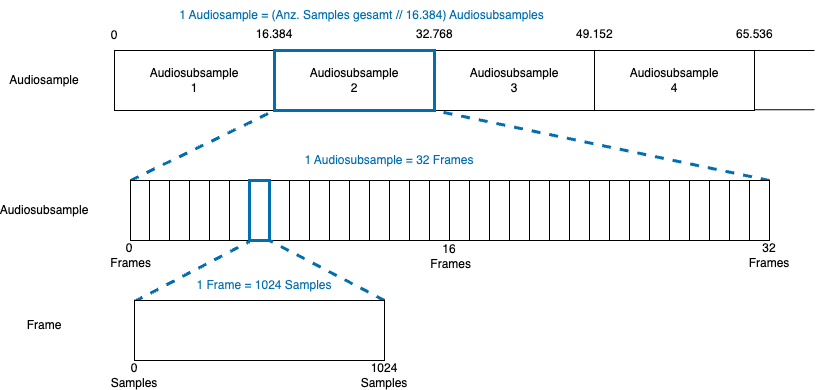
\includegraphics[width=0.8\textwidth]{images/08_durchfuehrung/audiosubsamples_frames_overview.png}
\caption{Darstellung der Unterteilung der Audiosamples in Audiosubsamples und Frames}
\label{fig:img-audiosubsamples-frames-overview}
\end{figure}

Das Sliding Window Prinzip, mit dem Audiosubsamples in überlappende Frames unterteilt werden, ist in \textbf{\autoref{fig:img-sliding-window}} dargestellt.

\begin{figure}[h!]
\centering
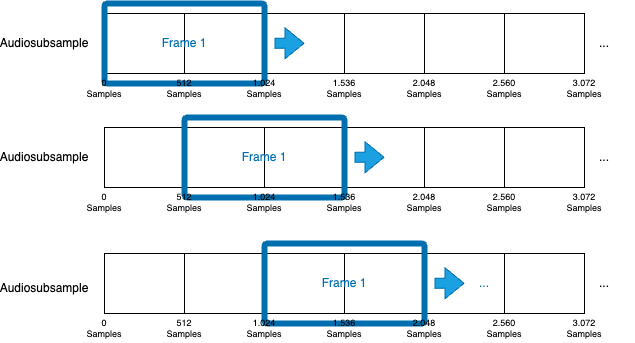
\includegraphics[width=0.7\textwidth]{images/08_durchfuehrung/sliding_window.png}
\caption{Darstellung des Sliding Window Prinzips}
\label{fig:img-sliding-window}
\end{figure}

Nun können die Mel-Spektrogramme erstellt werden. Eine Spalte des Spektrogramms wird dabei aus einem Frame berechnet. Setzt man die 32 in einem Audiosubsample enthaltenen Frames, also Spektrogramm-Spalten, zusammen, erhält man das 32x30 Pixel große Spektrogramm für ein Subsample.

Abschließend müssen die erhaltenen Daten standardisiert, also mittelwertfrei gemacht werden. Dies ist beim maschinellen Lernen üblich und sorgt dafür, dass das Modell schneller und effizienter konvergiert, indem es die Varianz in den Eingabedaten reduziert und eine gleichmäßige Verteilung der Werte gewährleistet. Damit diese Standardisierung später beim Einsatz des neuronalen Netzes auf dem Mikrocontroller nachgeahmt werden kann, werden die Werte des Scalers, der die standardisierten Werte berechnet, exportiert.


\subsubsection{Aufteilen der Eingabedaten in Trainings- Test und Validierungsdaten}

\subsubsection{Training des Neuronalen Netzes}

TODO:

- Topologie

- Trainignsparameter und warum (Adam (?), Learning Rate, no. epochs, etc.)

- erklären wann Training zu Ende

- accuracy bla graph

- confusion matrix

- model.h5

(und in Validierng einfach nur eigene samples eingeben und schauen bzw. hier drauf verweisen)




\subsubsection{Betrieb des Neuronalen Netzes auf dem STM32 Microcontroller}
TODO:

- wieder Datenvorverarbeitung

- Scaler

- Vorgehen Cube.AI (model.h5)

- Inference Zeit

- Verweis auf Validierungs-Kapitel


\begin{itemize}
    \item Implementierung der Komponenten:
    \begin{itemize}
        \item Ansätze/Methoden: Beschreibung der Ansätze und Methoden für jedes Teilprojekt
        \item Verwendete Komponenten: Detaillierte Beschreibung der verwendeten Komponenten
        \item Erkenntnisse während der Implementierung: Erfahrungen und Änderungen während der Implementierung und Begründung für Alternativen
    \end{itemize}
    \item Integration der Komponenten: Integration der Komponenten in das Gesamtsystem (aus zeitlichen Gründen nicht erfolgt)
\end{itemize}


\subsubsection{Downsampling für die Verarbeitung von Audio durch das Neuronalen Netzes}



\subsection{Audio Engine des Samplers}


Die Hauptfunktionalität eines Audiosamplers ist natürlich das Aufnehmen und Abspielen von Audiosamples. 

Der ausgesuchte PCM5102a Audio Codec bietet leider nur einen Ausgabestream, was eine Neubestellung eines Codecs mit In/Output Stream bedeuten würde, um auch die Aufnahme zu implementieren.

Angesichts des eh schon ambitionierten Featureumfangs und der damit verbundenen Zeitknappheit, wurde die also Aufnahmefunktion gekürzt, sodass der Prototyp zu einer reinen ``Sample-Playback`` Maschine wird. (TODO Verweis auf Lastenfall)


Das folgende Kapitel befasst sich mit der Implementierung und Ansteuerung der Audiowiedergabe über den Audio Codec.

Zunächst folgt eine Erläuterung des grundlegenden Signalfluss der Audioengine:

\subsubsection{Signalfluss der Audioengine}

Alle Audiosamples werden auf einer angeschlossen \textbf{SD Karte} persistent gespeichert. Diese werden dann immer stückweise mit dem \textbf{FATFS} Dateisystem, welches für eingebettete Systeme optimiert ist, in die Applikationslogik und somit den Audiopufferspeicher geladen. 

Von hier aus reicht die \textbf{DMA} den Buffer per \textbf{I2S} Protokoll an den \textbf{Audio Codec} weiter. 

Der Audio Codec wandelt die digitalen PCM Signale in eine analoges Signal mit Line-Level (TODO: Line Pegel elektrisch angeben).

\begin{figure}[h!]
	\centering
	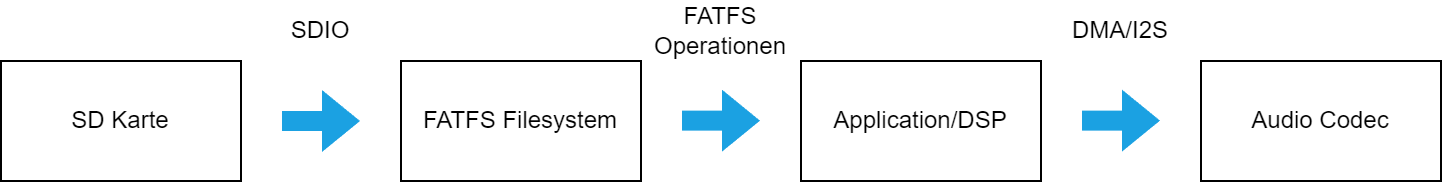
\includegraphics[width=0.6\textwidth]{images/08_durchfuehrung/audio/audio_signalflow.drawio.png}
	\caption{Digitaler Audio Signalfluss}
	\label{fig:audio_signalflow}
\end{figure}


\subsubsection{Latenzen}

TODO: TEST MIT MESSUNG IN TESTS (pulse an gpio geben, und audioausgang mit osci messen)

Echtzeitfähigkeit ist ein kritischer Aspekt bei elektronischen Audioinstrumenten. 
Eine niedrige Latenz ist entscheidend, um rhythmisch präzise und ``tight`` zu spielen, besonders wenn mehrere Instrumente miteinander synchronisiert werden müssen.

Die maximale Latenz, die ein menschlicher Profimusiker noch akzeptieren kann, liegt bei etwa 20ms. Diese Richtwert basiert auf der Wahrnehmungsgrenze, bei der Musiker und Live-Performern keine signifikante zeitliche Verzögerung zwischen dem Triggern eines Samples und dessen tatsächlichem Output am Ausgang spüren (https://www.highfidelity.com/backlog/how-much-latency-can-live-musicians-tolerate-da8e2ebe587a)

Um die Latenz auf ein Minimum zu reduzieren und sicherzustellen, dass elektronische Audioinstrumente reaktionsschnell und synchronisiert sind, können folgende Methoden angewendet werden:

\paragraph{Dimensionierung der Buffersize}\

Die erste Stellschraube ist die \textit{Buffersize}.
Das ist die Größe (in Bytes) des Audiobuffers.
Je kleiner der Audiobuffer, desto öfter pro Sekunde gibt die DMA dessen Inhalt an den Audio Codec weiter.

Das bringt jedoch auch Performanceeinbußen mit sich: Bei kleinen Audiobuffern hat die CPU, je nach Komplexität der durchzuführenden DSP-Operationen, möglicherweise nicht genug Zeit, um den gesamten Buffer zu verarbeiten.
Ein nur teils verarbeiteter Buffer kann hörbare Knackser und Störgeräusche am Ausgangssignal verursachen.

Hier gilt es also, die kleinstmögliche Buffersize zu ermitteln, ohne dass Störgeräusche auftreten.
Nach Experimentieren hat sich ein Wert von \textbf{128 Bytes} als adäquat herausgestellt.

\paragraph{Verwendung von Double Buffering}\

Double Buffering ermöglicht es, Daten in einem Pufferspeicher zu verarbeiten, während gleichzeitig ein anderer Puffer für die Eingabe oder Ausgabe verwendet wird. Dies reduziert Verzögerungen und ermöglicht eine nahtlose Datenverarbeitung, da der Prozessor nicht auf das Ende einer Übertragung oder Berechnung warten muss, bevor er fortfahren kann. (Quelle: https://www.eetimes.com/fundamentals-of-embedded-audio-part-3/)

\begin{figure}[H]
	\centering
	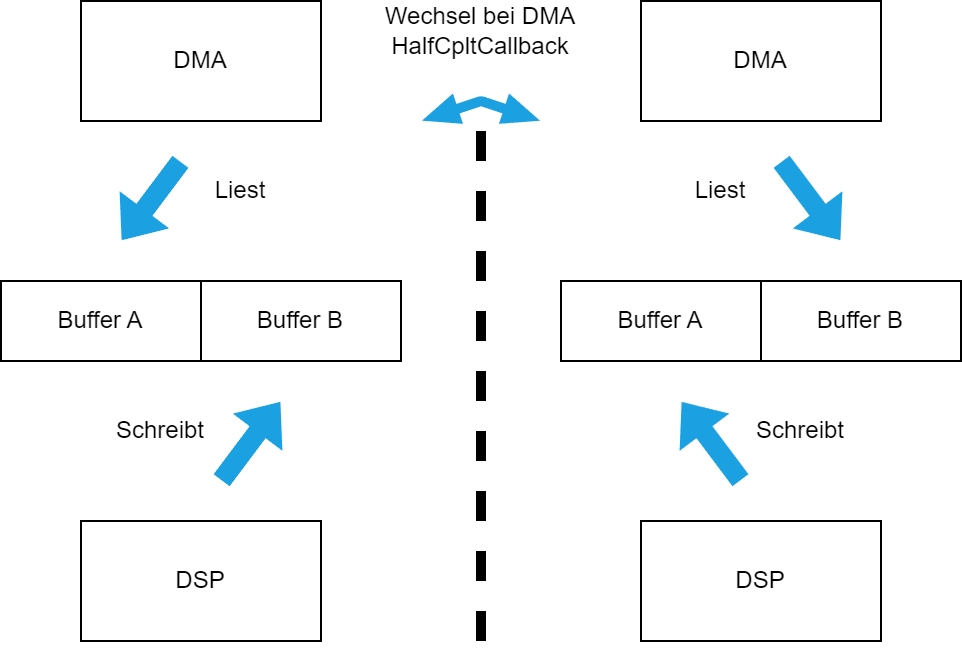
\includegraphics[width=0.6\textwidth]{images/08_durchfuehrung/audio/double_buffering.drawio.png}
	\caption{Double Buffering mit DMA und DSP}
	\label{fig:double_buffering}
\end{figure}


Bei I M A wird wird der Audiobuffer halbiert. 
Durch den Pointer \mintinline{c}|int16_t *outBufPtr| wird mit der DSP die Hälfte bearbeitet, die gerade nicht von der DMA übertragen wird.

In den Callback-Funktionen \mintinline{c}|HAL_I2S_TxHalfCpltCallback()| und \mintinline{c}|HAL_I2S_TxCpltCallback()| wird der Pointer auf die jeweilige Hälfte des Buffers, also auf (wie in  \textbf{\autoref{fig:double_buffering}} beschrieben:
\textbf{Buffer~A} und \textbf{Buffer~B}) gesetzt.


\inputminted[firstline=28, lastline=31]{c}{../../f401_sd_card_audio_codec_test/Core/Src/audio.c}

\inputminted[firstline=40, lastline=43]{c}{../../f401_sd_card_audio_codec_test/Core/Src/audio.c}


Diese Callbacks, werden automatisch aufgerufen, sobald die DMA die erste Hälfte, oder den gesamten Buffer übertragen hat. Sie eignen sich also sehr gut für die Setzung des Pointers.

Sobald das Flag \mintinline{c}|dma_dataReady == true| ist, wird die nächste Bufferhälfte von der SD Karte gelesen. 

\subsubsection{PCM5102a und I2S}

Ein sehr populäres Protokoll zur digitalen Audioübertragung ist I2S. Viele Codecs, so auch der PCM5102a unterstützen dieses Protokoll.

I2S (Inter-IC Sound) ist ein Standard für die digitale Übertragung von Audiodaten zwischen integrierten Schaltkreisen (ICs). Es wurde entwickelt, um die Kommunikation von digitalen Audiodaten zwischen verschiedenen Komponenten wie Mikrofonen, DACs (Digital-Analog-Wandler) und ADCs (Analog-Digital-Wandler) zu ermöglichen. 

TODO: PCM5102a Signale erklären (SCK, LCK, BCK, DIN)

Der PCM5102a erkennt komfortablerweise die eingehende Samplerate anhand der Bitclock.
Anders als bei vielen Audio Codecs ist keine zusätzliche Konfiguration des Chips über ein Kommunikationsprotokoll, wie I2C notwending.
Somit fallen auch keine Treiber für diesen Chip an.

- Der Einfachheit halber, festgelegte Samplerate und nur Stereo Samples! vllt eher zum DSP/Playback Part


\subsubsection{SD Karte}

Durch den sehr begrenzter RAM-Speicher des NUCLEO F401re Boards , ist es notwendig die Daten in Echtzeit von der SD-Karte zu streamen. Das setzt bei Stereo PCM Dateien, mit den gängigen Parametern, eine bestimmte Datenrate \( R \) voraus:

\begin{itemize}
	\item Abtastrate (Sampling Rate): 44.100 Hz (44,1 kHz)
	\item Bit-Tiefe: 16 Bit
	\item Kanäle: 2 (Stereo)
\end{itemize}


Die Datenrate \( R \) berechnet sich aus:

\[
R = \text{Sampling Rate} \times \text{Bit-Tiefe} \times \text{Anzahl der Kanäle}
\]



\[
R = 44{,}100 \, \text{Hz} \times 16 \, \text{bit} \times 2
\]

\[
R = 1{,}411{,}200 \, \text{bit/s} \approx 0.168 \, \text{MB/s}
\]


Theoretisch hätte eine Implementierung des FATFS-Dateisystems über SPI ausreichen müssen, um diese Datenraten zu bewältigen. 

Um die SDIO-Schnittstelle in das FATFS-Dateisystem zu integrieren, mussten zunächst Treiber entwickelt werden. Diese Treiber mappen die üblichen Dateioperationen wie \mintinline{c}|f_open()|, \mintinline{c}|f_read()| usw. über die SPI-Schnittstelle.


In der Praxis stellte sich jedoch heraus, dass der Audiobuffer nicht schnell genug gefüllt worden ist, was starke Knackser und Störgeräusche mit sich gebracht hat.

\begin{wrapfigure}{r}{0.3\textwidth} % Increase the width of the figure environment
	\vspace{-30pt + 0.02\textwidth}
	\hspace{0.02\textwidth} % Add horizontal space
	\fbox{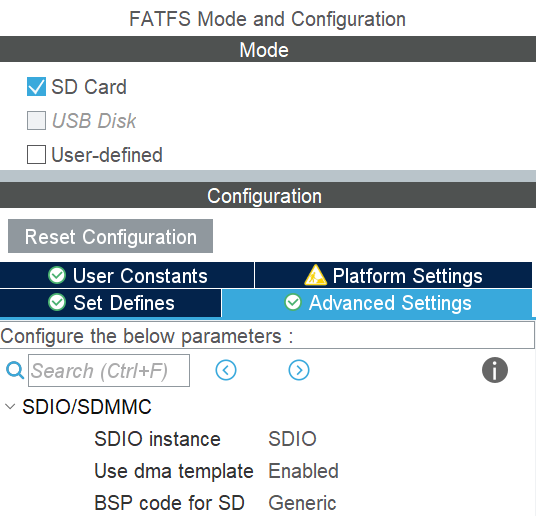
\includegraphics[width=0.28\textwidth]{images/08_durchfuehrung/audio/cubemx_sdio.png}}
	\caption{CubeMX FATFS SDIO Einbindung}
	\label{fig:cubemx_sdio}
\end{wrapfigure}

Dies erwies sich als äußerst vorteilhaft, da die SDIO-Implementierung zusammen mit FATFS direkt im Konfigurationstool von STM, \textbf{CubeMX}, ausgewählt werden kann. Die benötigten Treiber werden von CubeMX automatisch generiert und integrieren sich problemlos in das Dateisystem.

\subsubsection{Playback und Pitched Playback}


TODO Umsetzung im Code

CODE 

CODE 

CODE 

CODE 

CODE 

CODE 

CODE

CODE 




\newpage
\section{Test und Validierung}
\label{sec:test-validation}
Zur Überprüfung der Anforderungserfüllung jedes Lastenfalls (LF) wurden zunächst alle Komponenten einzeln entwickelt und getestet. Wie im \textbf{Abschnitt \ref{sec:no-gesamtintegration}} erläutert, verhinderten spezifische Herausforderungen eine Gesamtintegration der Systemkomponenten. Daher wurden keine Integrationstests entwickelt oder durchgeführt.

In den nachfolgenden Abschnitten werden die Testfälle und deren Ergebnisse für jeden Lastenfall beschrieben. Diese dienen dazu, die korrekte Funktionalität und die erfolgreiche Umsetzung der jeweiligen Anforderungen zu validieren.


\begin{itemize}
	\item Testfälle beschreiben, wurden LF erfüllt?
	\item Dokumentation des Tests und der Inbetriebnahme, Testprotokoll in der Form: Erwartetes Verhalten/gemessenes Verhalten, Checklisten
	\item Genau so wie in der ES Dokumentation
\end{itemize}

\textcolor{red}{TODO: Tests nach Redundanz aussortieren}
\textcolor{red}{TODO: Vorschlag Leon: Evtl. Struktur ändern? Ziel ist Validierung von LFs. In ES hatten wir ja keine LFs, daher mein Vorschlag: wie in SYP, also subsection: LF 01; subsubsection: Testen der korrekten Funktionsweise des Encoders, noch eine subsection für den zweiten Test für den LF (falls erforderlich) usw.}

\subsubsection{Testprotokoll: Latenzmessung}
\label{test-latenzmessung}

Messung der Latenz vom Zeitpunkt des Triggerinputs bis zur Audioausgabe über den Audio-Codec.

Durchführung mit dem STM32-Audioprojekt aus dem Repository (\href{run:../../f401_sd_card_audio_codec_test/}{\texttt{/f401\_sd\_card\_audio\_codec\_test/}}).
Der Audio-Codec, sowie der SD-Kartenleser müssen wie im Schaltplan(TODO: REFERENZ auf Schaltplan) verbunden werden.

\paragraph{Schritte:}
\begin{enumerate}
	\item Anschluss zweier Oszilloskop-Sonden: an Trigger-Input/Play-Button-Pin und Audio-Ausgang.
	\item Laden einer Test PCM .wav-Datei mit einer Samplerate von \SI{44.1}{\kilo\hertz}, 16 Bit und Stereo/2 Kanälen auf die SD-Karte.
	\item Umschalten des Oszilloskops in den Single-Shot-Modus und Konfiguration zur Auslösung durch den Audio-Kanal.
	\item Abspielen der Testdatei durch Auslösen des Play-Buttons.
	\item Positionierung zweier Mess-Cursor: einer auf die erste Flanke des Trigger-Input-Signals und der andere auf den Beginn des Audio-Ausgangssignals.
\end{enumerate}
\paragraph{Erwartete Werte}
	Die erwartet Latenz errechnet sich wie folgt:
	
	Gegeben:
	\begin{align*}
		\text{Samplerate} &= \SI{44.1}{\kilo\hertz} = 44{,}100 \, \text{Samples pro Sekunde} \\
		\text{Puffergröße} &= 256 \, \text{Samples}
	\end{align*}
	
	\paragraph*{Berechnung der Latenz}
	
	\[
	\text{Zeit pro Sample} = \frac{1 \, \text{Sekunde}}{44{,}100 \, \text{Samples}} \approx \SI{22.68}{\micro\second}
	\]
	
	\[
	\text{Zeit für einen Puffer} = 256 \, \text{Samples} \times \SI{22.68}{\micro\second} \approx \SI{5.8}{\milli\second}
	\]
	
	Die Latenz für ein System mit den angegebenen Parametern beträgt also etwa \( \SI{5.8}{\milli\second} \).
\paragraph{Testergebnisse}

\begin{itemize}
	\item Gemessene Latenz von \SI{6.4}{\milli\second} (\textbf{BX-AX} in Abbildung  \ref{fig:audio-latency-test}).
	\item Die Abweichung von der erwarteten Latenz ist wahrscheinlich auf die Verarbeitungszeiten des Audio-Codecs zurückzuführen sein.
	\item Sehr praktikabler Latenzwert für Audioinstrument.
\end{itemize}

\begin{figure}[H]
	\centering
	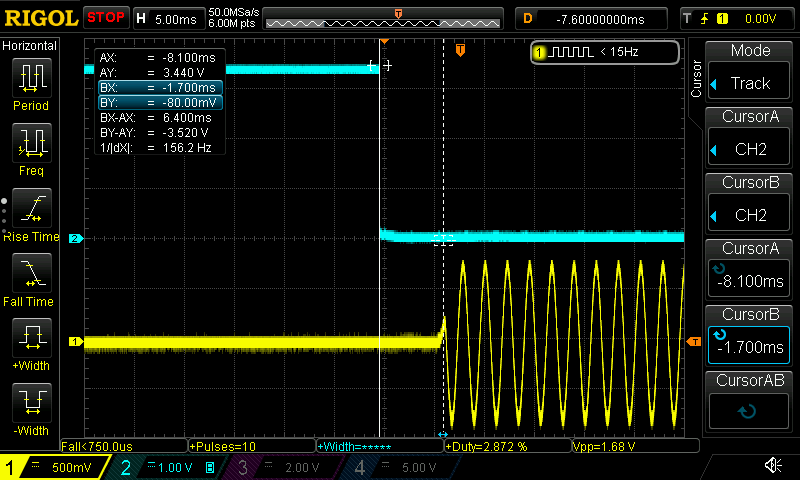
\includegraphics[width=0.6\textwidth]{images/10_test_validierung/audio/audio-latency-test.png}
	\caption{Latenzmessung von Trigger (Blau) bis Audioausgang (Gelb)}
	\label{fig:audio-latency-test}
\end{figure}

\subsubsection{Testprotokoll: /LFNeuronales Netz}
\label{test-latenzmessung}

\begin{itemize}
	\item Gemessene Latenz von \SI{6.4}{\milli\second} (\textbf{BX-AX} in Abbildung  \ref{fig:audio-latency-test}).
	\item Die Abweichung von der erwarteten Latenz ist wahrscheinlich auf die Verarbeitungszeiten des Audio-Codecs zurückzuführen.
	\item Sehr praktikabler Latenzwert für Audioinstrument.
\end{itemize}

\subsection{Testprotokoll: /LF01/}
\textbf{\hyperlink{LF01_Link}{LF01}} \\

\subsubsection{Auswertung der Drehung des Encoders}
\begin{itemize}
	\item \textbf{Testfall:} Prüfung des Drehverhaltens
	\item \textbf{Schritte:}
	\begin{enumerate}
		\item Der Encoder wird schnell und langsam in beide Richtungen gedreht.
		\item Dabei wird die Zählvariable \texttt{rotary\_enc\_count} beobachtet.
	\end{enumerate}
\item \textbf{Testergebnisse:}
\begin{itemize}
	\item Die Zählvariable zählt wie erwartet hoch und runter.
	\item Nur beim Betreten der \texttt{HAL\_GPIO\_EXTI\_Callback} soll die Variable hochgezählt werden.
\end{itemize}

\textbf{Gemessene Ergebnisse:}
\begin{itemize}
	\item Während der Tests wurde beobachtet, dass die Zählvariable korrekt hoch- und runtergezählt hat. Bei jeder Interaktion mit dem Encoder hat sich der Wert der Zählvariable entsprechend erhöht oder verringert.
	\item Die Zählvariable wurde ausschließlich beim Betreten der \texttt{HAL\_GPIO\_EXTI\_Callback} Funktion verändert. In allen anderen Fällen blieb die Zählvariable unverändert.
\end{itemize}

\begin{itemize}
	\item Es wurden keine Mehrfachauslösungen festgestellt. Jede Drehung des Encoders, sowohl schnell als auch langsam, führte zu einer einzigen Zähländerung, wie erwartet.
\end{itemize}

\end{itemize}




\textbf{Beschreibung des Vorgehens:}
Um das Drehverhalten des Encoders zu testen, würde de Encoder an das System angeschlossen und die Funktionalität überprüft. Anschließend haben wir den Encoder in beiden Richtungen, sowohl schnell als auch langsam, gedreht und die Zählvariable 
Die Zählvariable \texttt{rotary\_enc\_count} stand dabei unter Beobachtung, um sicherzustellen, dass sie ausschließlich durch die \texttt{HAL\_GPIO\_EXTI\_Callback} beeinflusst wird.


\subsubsection{Debouncing des Push-Buttons}
\begin{itemize}
	\item \textbf{Testfall:} Prüfung der Funktionalität des Push-Buttons.
	\item \textbf{Schritte:}
	\begin{enumerate}
		\item Erstellung einer Zähl Variable \boldinline{cnt}
		\item Drücken des Push-Button.
		\item Prüfen ob der Interrupt korrekt ausgelöst wird.
		\item Das korrekte Verhalten des Entprellen prüfen.
	\end{enumerate}
	\item \textbf{Erwartete Werte:}
	\begin{itemize}
		\item Der Interrupt wird bei jedem Drücken sauber und eindeutig ausgelöst.
		\item Es treten kein Prellen oder Mehrfachauslösungen auf.
	\end{itemize}
	\item \textbf{Testergebnisse:}
	\begin{itemize}
		\item Der Interrupt wurde bei jedem Drücken zuverlässig und eindeutig ausgelöst.
		\item Es traten keine Prellen oder Mehrfachauslösungen auf. Die \boldinline{cnt} hat korrekt hochgezählt.
	\end{itemize}
\end{itemize}


\textbf{Beschreibung des Vorgehens:}
Der Push-Button würde mehrmals gedrückt und dabei beobachtet, ob der Interrupt korrekt ausgelöst wurde. Während des Tests wird darauf geachtet, ob der Button prellte oder Mehrfachauslösungen verursachte in dem ein Zähl Variable \texttt{cnt} im Debugger beobachte würde. Die Ergebnisse bestätigten, dass der Interrupt zuverlässig und ohne Prellen funktionierte.

\subsubsection{Menünavigation}
\begin{itemize}
	\item \textbf{Testfall:} Testen der Navigation im Menü mithilfe des Encoders.
	\item \textbf{Schritte:}
	\begin{enumerate}
		\item Den Encoder wird in beide Richtungen gedreht und die Cursor-Bewegung beobachtet. Die cursor Variable \texttt{cursor\_index} des Filemanagers  im Debugger prüfen auf deren Zählverhalten.
		\item Der Push-Button wird gedrückt, um eine Auswahl zu treffen. Der Flag switch\_push\_button prüfen um die Validierung des korrekten Verhaltens beim drücken zu bestätigen.
	\end{enumerate}
	\item \textbf{Erwartete Werte:}
	\begin{itemize}
		\item Der Cursor bewegt sich entsprechend der Drehrichtung des Encoders.
		\item Die Auswahl wird korrekt angezeigt, wenn der Push-Button gedrückt wird.
	\end{itemize}
	
	\item \textbf{Testergebnisse:}
	\begin{itemize}
		\item Der Cursor bewegte sich korrekt und präzise entsprechend der Encoder-Drehung.
		\item Die Auswahl wurde zuverlässig angezeigt, nachdem der Push-Button gedrückt wurde.
	\end{itemize}
\end{itemize}

\textbf{Beschreibung des Vorgehens:} 
Der Encoder wird gedreht, um sicherzustellen, dass der Cursor im Menü korrekt bewegt wird. Die Cursor Variable \texttt{cursor\_index} im FileManager Struct \texttt{fm} wird korrekt hoch und runter gezählt bei entsprechender Bewegung. Anschließend habe ich den Push-Button betätigt, um zu prüfen, ob die Auswahl entsprechend angezeigt wird.  Der Flag \texttt{switch\_push\_button} würde ebenfalls korrekt gesetzt.

\subsection{Testprotokoll: /LF02/}
\textbf{\hyperlink{LF02_Link}{LF02}} \\

\subsubsection{ADC-Konfiguration überprüfen}
\begin{itemize}
	\item \textbf{Testfall:} Überprüfung der ADC-Konfiguration.
	\item \textbf{Schritte:}
	\begin{enumerate}
		\item Die Auflösung, Sample-Rate und Referenzspannung des ADCs wurden überprüft.
		\item Es wird sichergestellt, dass der ADC korrekt konfiguriert ist.
		\item Die Referenzspannung wird mit einem Multimeter gemessen, um ihre Übereinstimmung mit den Werte im Debugger zu bestätigen.
		\item Die Sample-Rate wird durch Analyse der ADC-Konfigurationsregister überprüft und mit den erwarteten Werten verglichen. \texttt{ADC1\_CFGR} Configuration Register.
	\end{enumerate}
	\item \textbf{Erwartete Werte:}
	\begin{itemize}
		\item Auflösung: 12-bit (0-4096 Werte).
		\item Sample-Rate entspricht den Spezifikationen.
		\item Referenzspannung entspricht der spezifizierten Spannung.
	\end{itemize}
	\item \textbf{Testergebnisse:}
	\begin{itemize}
		\item Die Auflösung des ADCs wurde korrekt auf 12-bit (0-4096 Werte) eingestellt.
		\item Die Referenzspannung wurde mit einem Multimeter gemessen und entsprach der spezifizierten Spannung.
		\item Die Sample-Rate wurde durch Überprüfung der ADC-Konfigurationsregister bestätigt und entsprach den angegebenen Spezifikationen.
		\item Die ADC-Konfiguration war ordnungsgemäß und entsprechend den Anforderungen eingerichtet.
	\end{itemize}
\end{itemize}

\textbf{Beschreibung des Vorgehens:}
Die Konfiguration des ADCs wurde durch Überprüfung der Auflösung, Sample-Rate und Referenzspannung sichergestellt. Die Referenzspannung wurde direkt mit einem Multimeter gemessen, um ihre Übereinstimmung mit den Spezifikationen zu bestätigen. Die Sample-Rate wurde durch die Analyse der ADC-Konfigurationsregister verifiziert, indem die tatsächliche Rate mit den erwarteten Werten verglichen wurde. Die Validierung erfolgte durch den Einsatz eines Debugging-Tools, um zu gewährleisten, dass der ADC gemäß den Anforderungen konfiguriert ist.


\subsubsection{DMA-Konfiguration überprüfen}
\begin{itemize}
	\item \textbf{Testfall:} Überprüfung der DMA-Konfiguration.
	\item \textbf{Schritte:}
	\begin{enumerate}
		\item Es wird sichergestellt, dass der DMA die ADC-Daten in den Puffer \texttt{currentValues} überträgt.
		\item Die Übertragungsart und die Übertragungsrate werden überprüft.
		\item Das Datenformat wird auf WORD (16-Bit) konfiguriert und geprüft.
	\end{enumerate}
	\item \textbf{Erwartete Werte:}
	\begin{itemize}
		\item Korrekte Konfiguration des DMA, Übertragungsmodus auf Circular.
		\item Datenformat korrekt auf WORD (16-Bit) eingestellt.
	\end{itemize}
	\item \textbf{Testergebnisse:}
	\begin{itemize}
		\item Der DMA überträgt die ADC-Daten wie erwartet in den Puffer \texttt{currentValues}.
		\item Die Übertragungsart ist korrekt auf Circular eingestellt.
		\item Das Datenformat wurde erfolgreich auf WORD (16-Bit) konfiguriert. Die Überprüfung wurde durch Einsicht in die DMA-Register bestätigt. Insbesondere wurden die Registerwerte für `PSIZE` und `MSIZE` auf 16-Bit überprüft, um die korrekte Einstellung des Datenformats zu bestätigen.
	\end{itemize}
\end{itemize}


\textbf{Beschreibung des Vorgehens:}
Die DMA-Konfiguration wurde überprüft, indem zuerst sichergestellt wurde, dass der DMA die ADC-Daten korrekt in den Puffer \texttt{currentValues} überträgt(Debugging). Danach wurde die Übertragungsart auf Circular gesetzt und die Übertragungsrate validiert. Schließlich wurde das Datenformat auf WORD (16-Bit) konfiguriert und durch Einsicht in die entsprechenden DMA-Register überprüft, insbesondere durch Überprüfung der Registerwerte für `PSIZE` und `MSIZE`.

\subsubsection{Daten analysieren}
\begin{itemize}
	\item \textbf{Testfall:} Analyse der aufgezeichneten ADC-Werte und Prüfung der Glättung.
	\item \textbf{Schritte:}
	\begin{enumerate}
		\item Die ADC-Werte \texttt{fm.fader\_Class[]}, \texttt{adcBuffer[]}, \texttt{smoothValue[]} und \texttt{currentClassPercentADC[]} werden mit einem Debugger analysiert.
		\item Es wird geprüft, ob eine lineare Zunahme der Werte entsprechend der Stellung des Schiebe-Potentiometers vorliegt.
		\item Der \texttt{smoothValue[]} wird berechnet, und es wird auf Schwankungen und plötzliche Änderungen geprüft. Glättung erfolgt mit \texttt{100, 1000, 10000, 30000, 100000} aufeinander addierten Werten.
	\end{enumerate}
	\item \textbf{Erwartete Werte:} 
	\begin{itemize}
		\item ADC-Werte entsprechen den Positionen des Potentiometers.
		\item Die geglätteten Werte zeigen eine stabile Wertentwicklung.
		\item Keine unerwarteten Sprünge oder signifikanten Schwankungen; Grundrauschen um wenige Volt ist normal.
	\end{itemize}
	\item \textbf{Testergebnisse:}
	\begin{itemize}
		\item Die ADC-Werte \texttt{fm.fader\_Class[]}, \texttt{adcBuffer[]}, \texttt{smoothValue[]} und \texttt{currentClassPercentADC[]} wurden erfolgreich mit dem Debugger analysiert.
		\item Die Werte zeigten eine erwartungsgemäße lineare Zunahme in Abhängigkeit von der Potentiometer-Position.
		\item Der \texttt{smoothValue[]} zeigte eine stabile Wertentwicklung ohne signifikante Schwankungen oder plötzliche Änderungen.
		\item Es traten keine unerwarteten Sprünge auf. Ein sehr geringes Grundrauschen wurde erstmal als normal eingestuft.\textbf{30000} aufeinader addierte Werte dessen Mittelwert berechnet würde stellten sich jedoch am als Effzietesten raus.
	\end{itemize}
\end{itemize}

\textbf{Beschreibung des Vorgehens:}
Die ADC-Werte wurden mit einem Debugger analysiert, um sicherzustellen, dass sie der Stellung des Potentiometers entsprechen. Es wurde überprüft, ob die Werte linear ansteigen und ob der geglättete Wert \texttt{smoothValue[]} stabil bleibt. Schwankungen und plötzliche Änderungen wurden geprüft, um die Effektivität der Glättung zu bewerten. Das Grundrauschen wurde als normal eingestuft.

\textbf{Lösung um das Grundrauschen zu minimieren:}
Das Grundrauschen könnte zukünftig durch den Einsatz von Kondensatoren, z.B. 100 nF, minimiert oder beseitigt werden.

\newpage
\subsubsection{Wiedergabe der Fader-Werte und Filterung auf dem Display}

\begin{itemize}
	\item \textbf{Testfall:} Überprüfung der korrekten Anzeige der Fader-Werte und der Filterung der Samples auf dem Display.
	\item \textbf{Schritte:}
	\begin{enumerate}
		\item Fader-Werte anzeigen:
		\begin{enumerate}
			\item Bewege die Schiebepotentiometer (Fader) zyklisch.
			\item Überprüfe, ob die prozentualen Werte der Potentiometer korrekt und in Echtzeit auf dem Display angezeigt werden.
			\item Vergewissere dich, dass die angezeigten Werte die richtige Spannung und die korrekte Zuordnung zu den Klassen (wie Rhythmic, Sustained, usw.) widerspiegeln.
		\end{enumerate}
		\item Filterung der Samples:
		\begin{enumerate}
			\item Bewege die Schiebepotentiometer und stelle den Schwellenwert für die Filterung ein.
			\item Überprüfe, ob die Liste der Samples auf dem Display dynamisch aktualisiert wird und nur die Samples anzeigt, deren Audio-Klassen nach der Klassifizierung den Schwellenwert nicht überschreiten.
			\item Teste verschiedene Schwellenwerte und überprüfe, ob die angezeigten Samples korrekt gefiltert werden.
		\end{enumerate}
	\end{enumerate}
	\item \textbf{Erwartete Ergebnisse:}
	\begin{itemize}
		\item Die prozentualen Werte der Fader werden korrekt und in Echtzeit auf dem Display angezeigt.
		\item Die Klassen der Potentiometer-Einstellungen werden korrekt auf dem Display angezeigt.
		\item Die Liste der Samples wird dynamisch und korrekt basierend auf den Potentiometer-Werten und dem Schwellenwert aktualisiert.
		\item Keine Anzeigeprobleme oder Verzögerungen bei der Aktualisierung des Displays.
	\end{itemize}
	\item \textbf{Testergebnisse:}
	\begin{itemize}
		\item Die prozentualen Fader-Werte wurden korrekt auf dem Display angezeigt und spiegelten die realen Werte der Potentiometer wider.
		\item Die Filterung der Samples funktionierte wie erwartet; nur die Samples, die den eingestellten Schwellenwert erfüllten, wurden angezeigt.
		\item Die Anzeige auf dem Display war frei von Verzögerungen oder Fehlern.
	\end{itemize}
\end{itemize}



\subsection{Testprotokoll: LF01 LF02 SD-Karten SPI-Schnittstelle}
\textbf{\hyperlink{LF01_Link}{LF01}} \\
\textbf{\hyperlink{LF02_Link}{LF02}} \\
\subsubsection{Testzielsetzung}
Dieser Test überprüft die Funktionalität der Lese- und Schreibfunktionen für die SD-Karte über die SPI-Schnittstelle.

\subsubsection{Testdurchführung}

\begin{itemize}
	\item \textbf{Mounten des Dateisystems:}
	\begin{itemize}
		\item Die Funktion \texttt{f\_mount} wurde aufgerufen, um das Dateisystem der SD-Karte zu mounten.
		\item Der Rückgabewert (\texttt{fres}) wurde überprüft. Im Fehlerfall wurde eine Meldung ausgegeben und der Test abgebrochen.
	\end{itemize}
	
	\item \textbf{SD-Karten-Statistiken:}
	\begin{itemize}
		\item Die Funktion \texttt{f\_getfree} wurde aufgerufen, um die freien Cluster, freien Sektoren und Gesamtsektoren der SD-Karte zu ermitteln.
		\item Im Fehlerfall wurde eine Meldung ausgegeben und der Test abgebrochen.
		\item Die Gesamt- und freien Speicherplatzwerte wurden berechnet und über \texttt{myprintf} ausgegeben.
	\end{itemize}
	
	\item \textbf{Lesen einer Datei:}
	\begin{itemize}
		\item Die Datei \texttt{test.txt} wurde mit der Funktion \texttt{f\_open} im Lesemodus geöffnet.
		\item Der Rückgabewert (\texttt{fres}) wurde überprüft. Im Fehlerfall wurde eine Meldung ausgegeben und der Test abgebrochen.
		\item Es wurde versucht, 30 Bytes aus der Datei zu lesen (\texttt{f\_gets}).
		\item Gelingt das Lesen, wurde der Inhalt der gelesenen Daten über \texttt{myprintf} ausgegeben.
		\item Im Fehlerfall wurde eine Meldung ausgegeben.
		\item Die Datei wurde mit \texttt{f\_close} geschlossen.
	\end{itemize}
	
	\item \textbf{Schreiben einer Datei:}
	\begin{itemize}
		\item Die Datei \texttt{write.txt} wurde mit der Funktion \texttt{f\_open} im Schreibmodus und mit Flags zum Anlegen der Datei geöffnet.
		\item Der Rückgabewert (\texttt{fres}) wurde überprüft. Im Fehlerfall wurde eine Meldung ausgegeben.
		\item Ein String (\texttt{"a new file is made!"}) wurde in den Puffer \texttt{readBuf} kopiert.
		\item Die Daten aus \texttt{readBuf} wurden mit \texttt{f\_write} in die Datei geschrieben.
		\item Die Anzahl der geschriebenen Bytes wurde über \texttt{myprintf} ausgegeben.
		\item Im Fehlerfall wurde eine Meldung ausgegeben.
		\item Die Datei wurde mit \texttt{f\_close} geschlossen.
	\end{itemize}
	
	\item \textbf{Dismounten des Dateisystems:}
	\begin{itemize}
		\item Die Funktion \texttt{f\_mount} wurde mit \texttt{NULL} aufgerufen, um das Dateisystem der SD-Karte zu dismounten.
	\end{itemize}
\end{itemize}

\subsubsection{Auswertung}
Der Test verlief erfolgreich:

\begin{itemize}
	\item Das Mounten und Dismounten des Dateisystems wurden erfolgreich durchgeführt.
	\item Die SD-Karten-Statistiken stimmten mit den Erwartungen überein.
	\item Das Lesen und Schreiben von .txt Dateien funktionierte einwandfrei.
\end{itemize}

Es wurde festgestellt, dass das Schreiben eines `struct` nicht möglich war. Eine zukünftige Lösung wird angestrebt.


\newpage
\section{Fazit}
\begin{itemize}
    \item Erkenntnisse und Gelerntes
\end{itemize}

Im Rahmen des Projekts konnten die in der Vorlesung ``Embedded Systems`` (ES) erlernten Kenntnisse weiter vertieft und erweitert werden. Das eigenständige Entwickeln eines Systems von der Idee über die Konzeption bis hin zur Umsetzung ermöglichte es, spezialisiertes Wissen und wertvolle Erfahrungen in den jeweiligen Interessensbereichen zu sammeln. Trotz der Herausforderung, teils komplexe Sachverhalte zu lösen, wurde ein tiefgreifendes Verständnis für die praktische Anwendung der verwendeten Technologien gefördert.


\textbf{TODO weiter schreiben, hab gerademkeine Zeit mehr :((}


\newpage
\printbibliography[title=Literaturverzeichnis]
\newpage


\appendix
\label{sec:appendix}

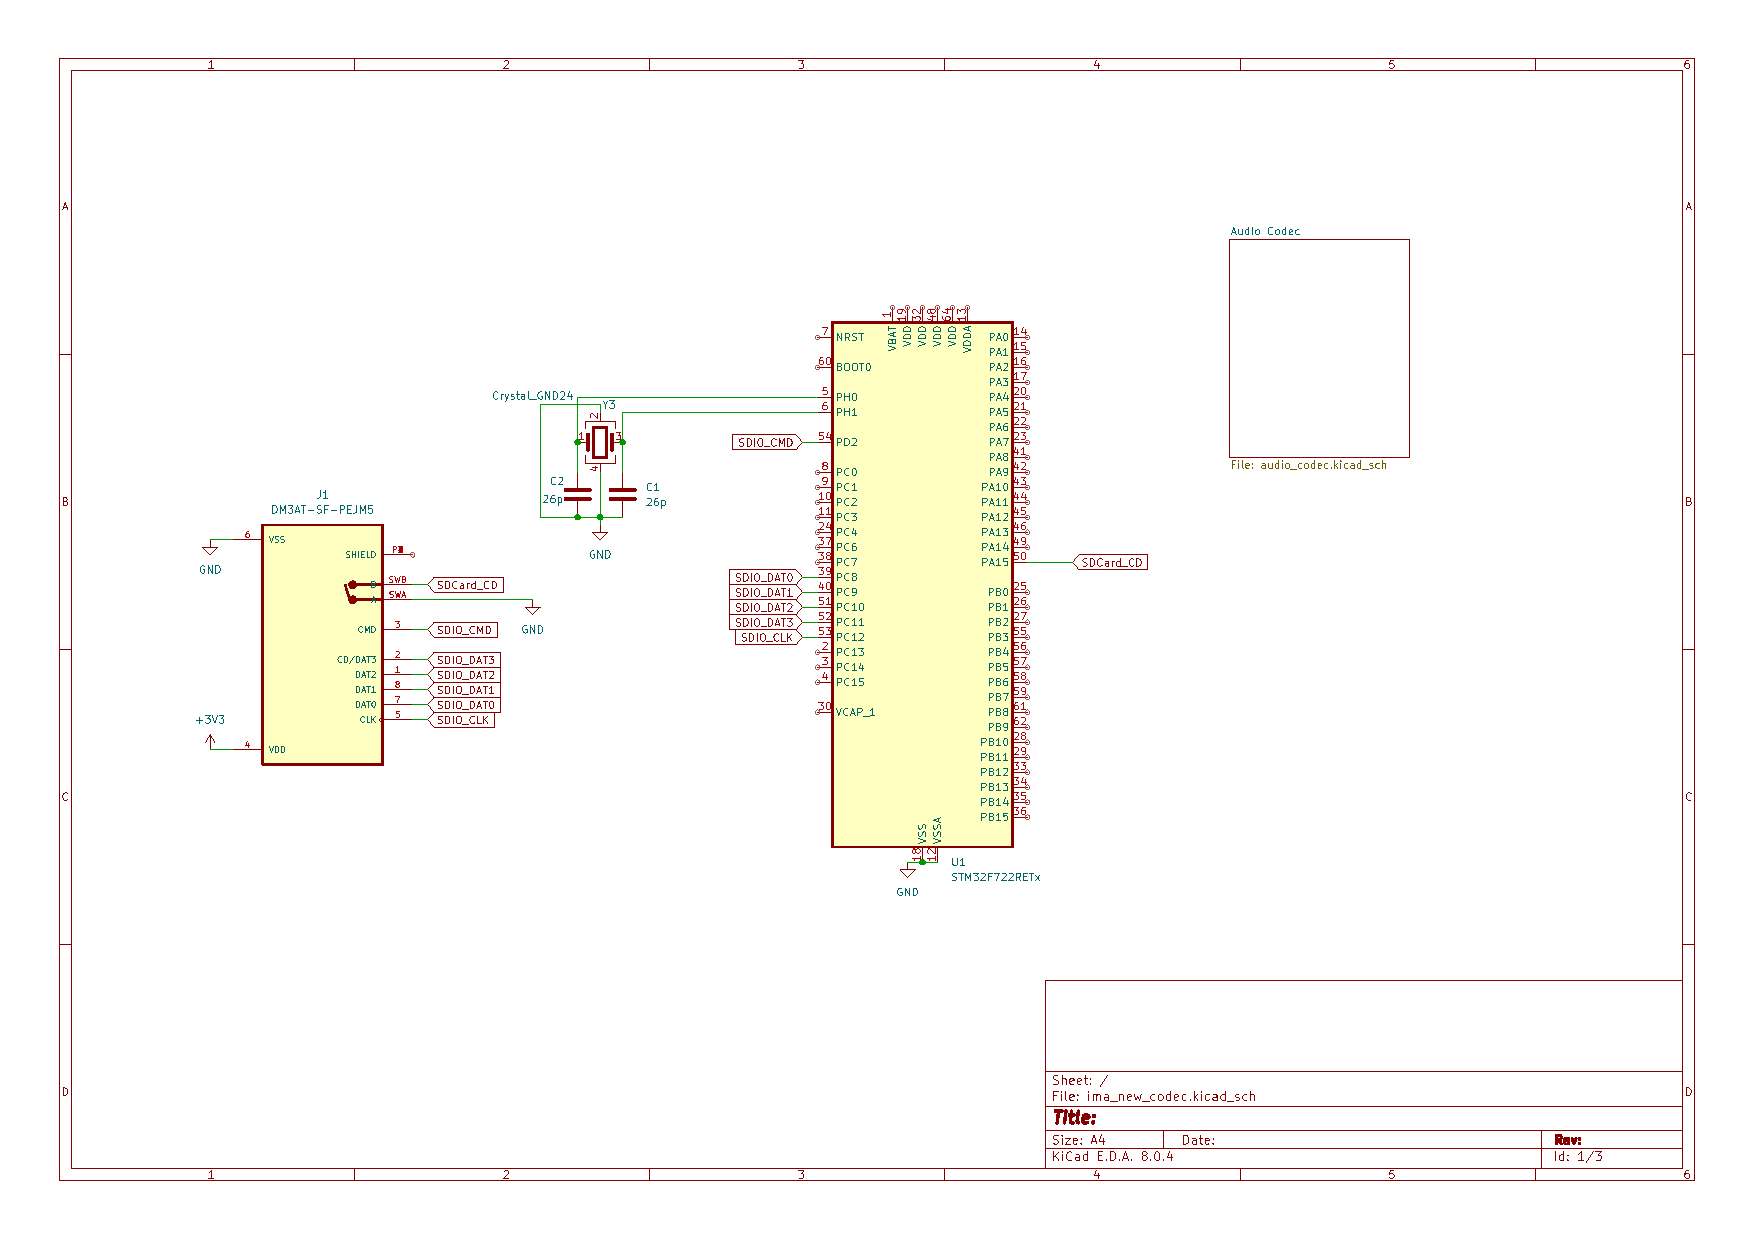
\includepdf[pages=-, landscape=true]{../schematics/ima_pcb_design.pdf}
\newpage

\end{document}